\documentclass[beamer=true]{standalone}
\usepackage{preamblesnotes}

\begin{document}
\settitle{光的反射現象Reflection of light}{光學第一課}{周末班}
\begin{frame}{光束和光線Light beam and light ray}
    \begin{figure}
        \centering
        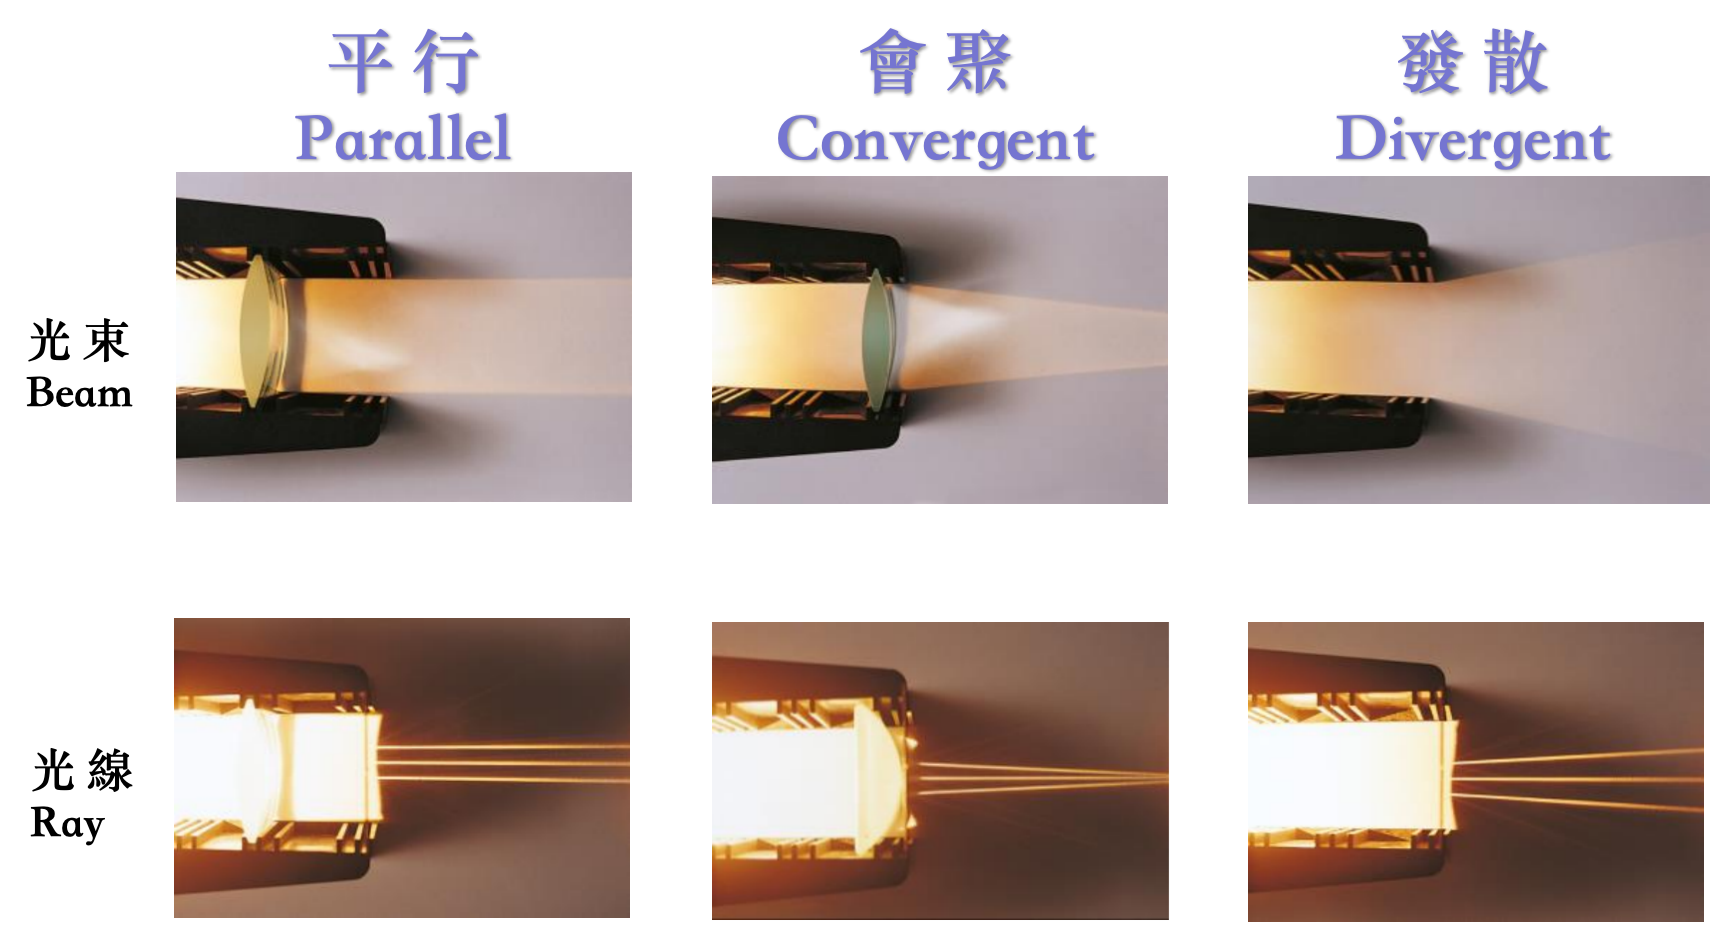
\includegraphics[width=1\linewidth]{assets/dwepdowedewdkewkge.png}
        
        
    \end{figure}
\end{frame}

\begin{frame}{光線圖Ray diagram}
\begin{itemize}
    \item 在光線圖中,\\In a ray diagram,
    \begin{itemize}
        \item 直線  表示光線的傳播路徑\\Solid line represents the path of light ray.
        \item 箭號表示光線的傳播方向\\Arrow represents the direction of travel.
    \end{itemize}
\end{itemize}\medskip
\begin{figure}
    \centering
    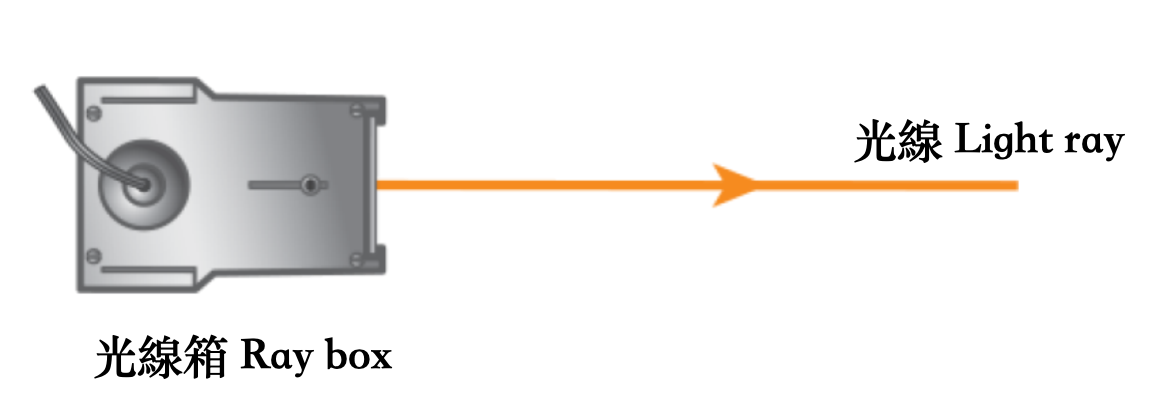
\includegraphics[width=0.666\linewidth]{assets/djdjweodjowiediowejdioew.png}
\end{figure}
\end{frame}

\begin{frame}{光錐Light cone}
    \begin{itemize}
        \item 來自點物體,到達眼睛的光會形成光錐。\\Rays from a point object to eye form a light cone.
    \end{itemize}\bigskip
\begin{figure}
    \centering
    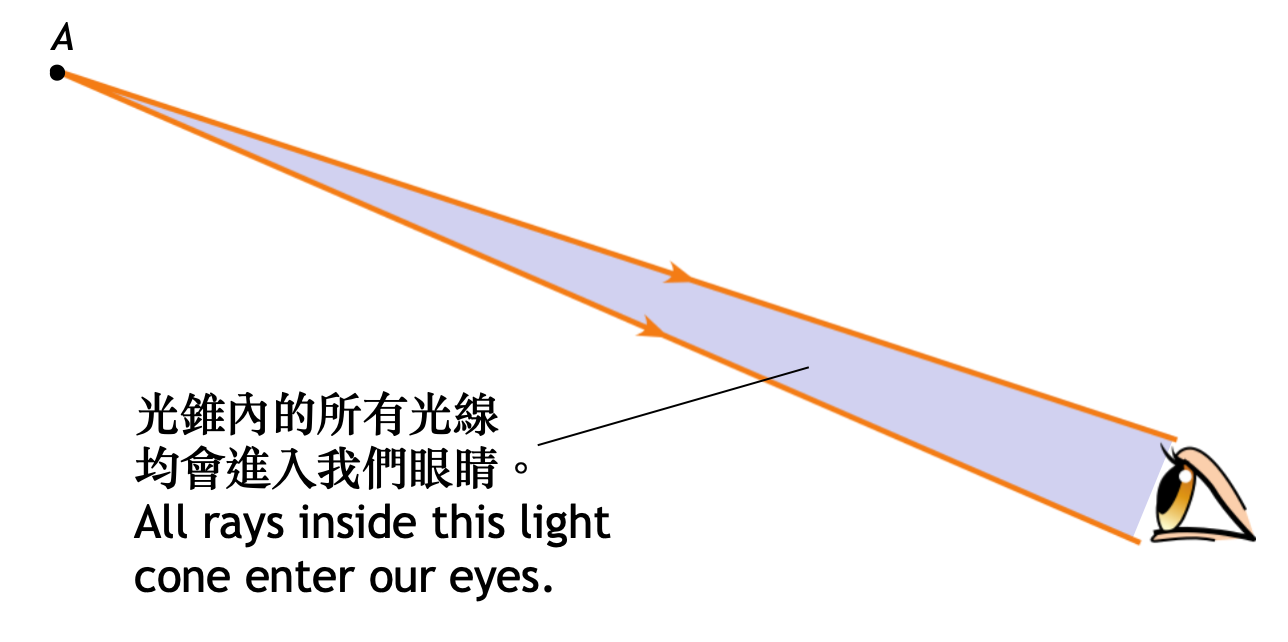
\includegraphics[width=0.6\linewidth]{assets/qwdoiwjidwqiodjioqwdijoqwjdo.png}
    
    
\end{figure}
    
\end{frame}

\begin{frame}{光錐Light cone}
\begin{itemize}
    \item 來自大型物體,需繪畫兩個來自物體端點的光錐\\For a large object, draw a light cone from each tip of the object.
\end{itemize}\bigskip
    \begin{figure}
        \centering
        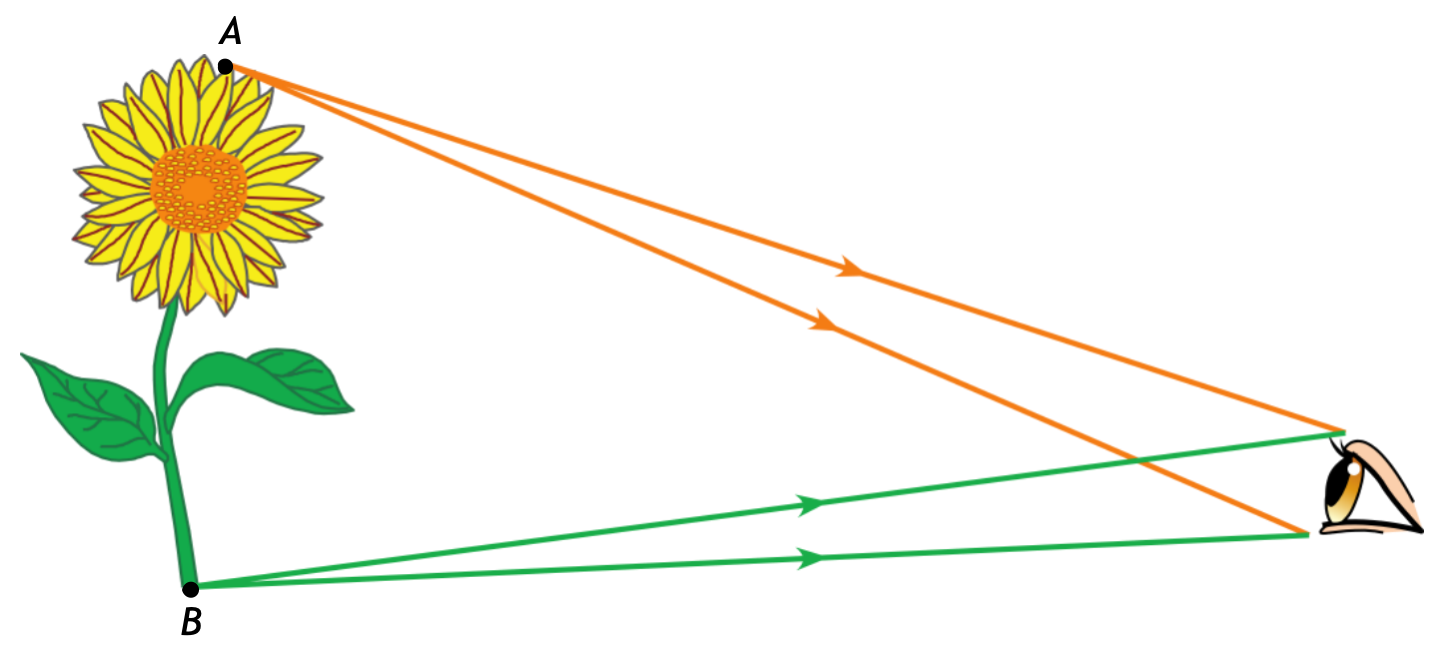
\includegraphics[width=0.75\linewidth]{assets/dwqdjwqdiwqjdoiqwoi1.png}
    \end{figure}
\end{frame}


\begin{frame}{發光及非發光體Luminous and non-luminous object}
    \begin{itemize}
        \item 發光體:能夠發光\\Luminous objects: emit light
        \item 不發光體:不能夠發光\\Non-luminous objects: do not emit light
    \end{itemize}\bigskip
    \begin{figure}
        \centering
        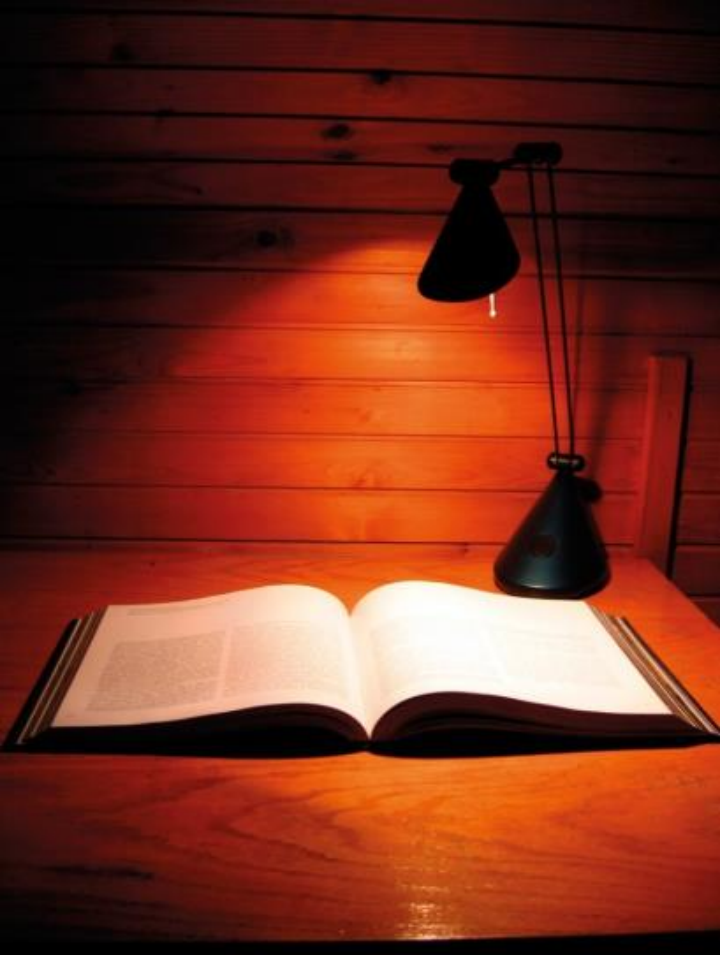
\includegraphics[width=0.25\linewidth]{assets/deowjdjdoijoidjowdqwp.png}
    \end{figure}
\end{frame}

\begin{frame}{光的反射Reflection of light}
    \begin{figure}
        \centering
        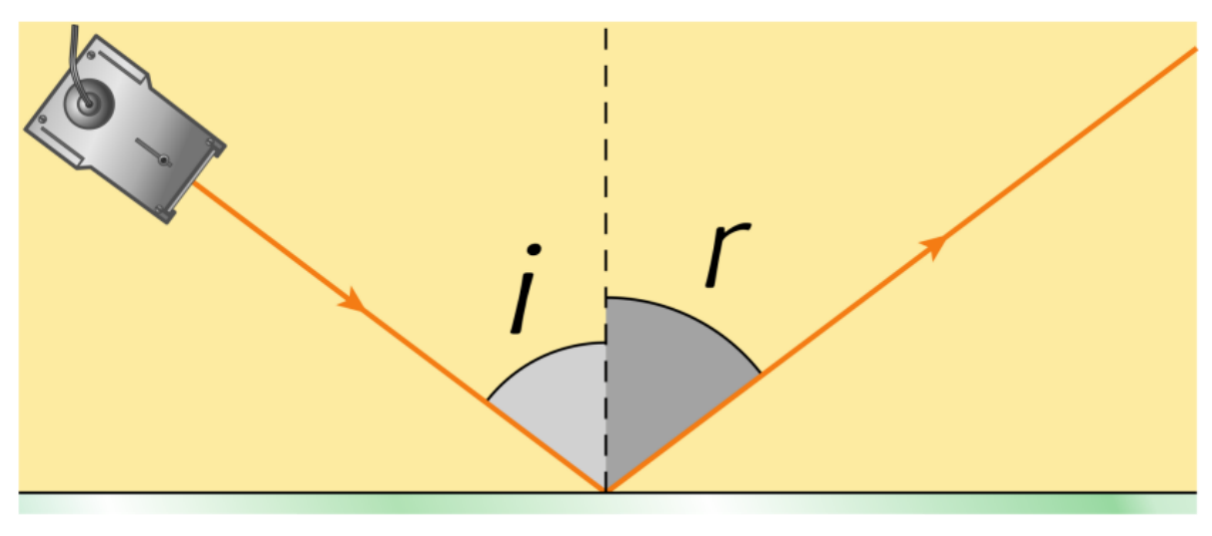
\includegraphics[width=0.45\linewidth]{assets/djoiqdqwiodijqwodage.png}
        
    \end{figure}
    \begin{figure}
        \centering
        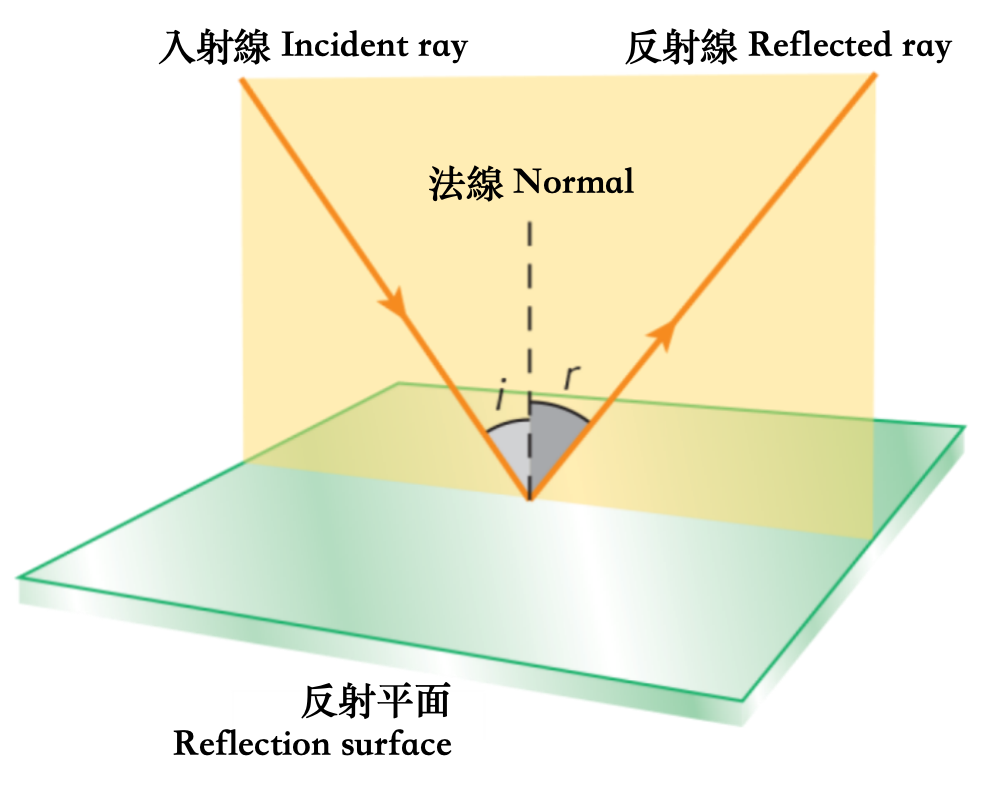
\includegraphics[width=0.58\linewidth]{assets/qdqwdiwqoe.png}
        
        
    \end{figure}
    
\end{frame}

\begin{frame}{光的反射Reflection of light}
    
    \begin{itemize}
        \item 當光線射到一個表面上,反射會發生。\\When a light ray is incident onto a surface, reflection occurs.
        \item 光線的傳播方向經常用法線作為參考表示。\\A normal can be drawn to indicate the orientation of the surface.
        \begin{itemize}
            \item 法線永遠垂直於表面切線。\\Normal is always perpendicular to tangent of a surface.
        \end{itemize}
        \item 入射光線與法線的角度稱為入射角$i$。\\The angle between the incident ray and the normal is the incident angle $i$.
        \item 反射光線與法線的角度稱為反射角$r$。\\The angle between the reflected ray and the normal is the reflected angle $r$.
    \end{itemize}
\end{frame}



\begin{frame}{反射定律定義Definition of law of reflection}
    \begin{alertblock}
        {反射定律Law of reflection}
        \begin{itemize}
        \setlength{\itemsep}{.6em}
            \item 反射角等於入射角。\\The angle of reflection is equal to the angle of incidence, \medskip
            \begin{equation}
                \therefore i=r
            \end{equation}
            \item 入射角、法線和反射角都必定在同一平面上。\\The incident ray, the normal and the reflected ray all lie in the same plane.
        \end{itemize}
    \end{alertblock}

    
\end{frame}


\begin{eg}
下圖顯示了一束光線入射到一個鏡子系統,該系統由兩個互相成直角的平面鏡組成。\\The following diagram shows a ray of light incident onto a mirror system which are set by two plane mirrors at right angle to each other.
{\par
    \centering
    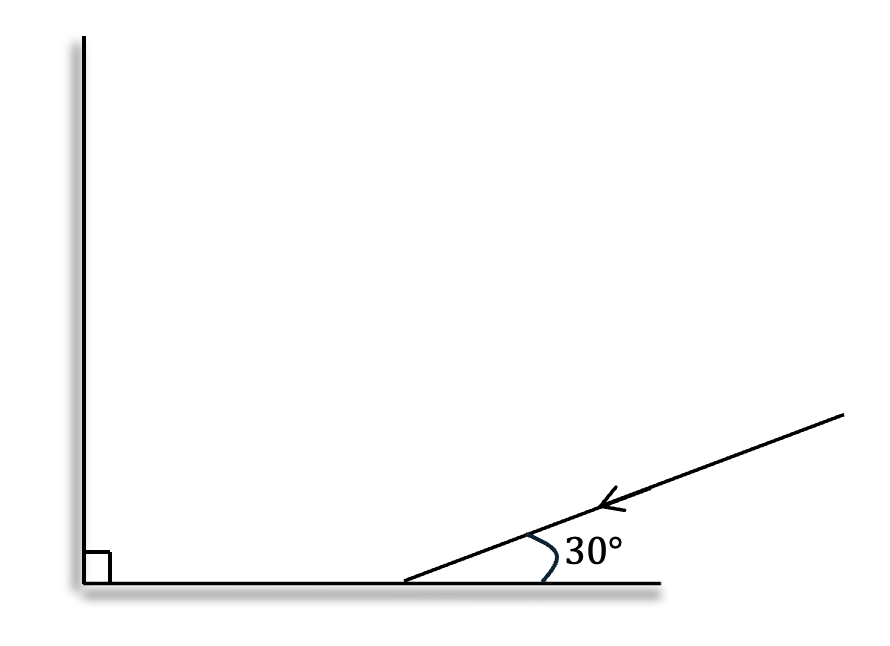
\includegraphics[width=0.4\linewidth]{assets/diqwdowqjdiojwqimage.png} 
\par}
\begin{itemize}
    \item [(a)] 從光線進入系統到離開系統的過程中,畫出光線的路徑。在圖中清楚標示入射角和反射角。\\Sketch the light rays until it leaves the system. Label angle of incidence and reflection clearly in the diagram.
\end{itemize}      
\end{eg}
\begin{eg}
    \begin{itemize}
        \item [(b)] 光線一共經歷了多少次反射?\\How many reflection that the ray undergoes in the process?\vspace{1cm}
        \item [(c)] 在最後一次反射時,反射角是多少?\\What is the angle of reflection at the last reflection?
    \end{itemize}
\end{eg}
\begin{eg}
    \begin{itemize}
        \item [(d)] 如果入射光線的角度為\dg{40},而不是 \dg{30},求最後一次反射時反射角。\\If the incident ray makes an angle of \dg{40} instead of \dg{30}. Find the angle of reflection of the last reflection.
    \end{itemize}
\end{eg}

\begin{eg}
    一束光線射向一個平面鏡,如圖所示。現在將平面鏡順時針旋轉 \dg{15}。\\A light ray is directed to a plane mirror as shown in the figure. Now the plane mirror is rotated clockwise for \dg{15}.
    \begin{figure}[h]
        \centering
        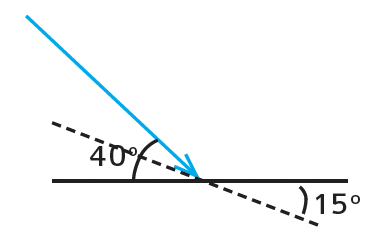
\includegraphics[width=0.3\linewidth]{assets/dwdop12age.png}
    \end{figure}
    \begin{itemize}
        \item [(a)] 寫出法線旋轉的角度。\\Write down the rotation angle of normal of mirror reflected.
    \end{itemize}
    
\end{eg}
\begin{eg}
    \begin{itemize}
        \item [(b)] 寫出新的入射角和反射角。\\Write down the new angle of incidence and reflection.\vspace{2cm}
        \item [(c)] 寫出反射角旋轉的角度。\\Write down the angle that the reflected ray rotated.
    \end{itemize}
\end{eg}
\begin{eg}
根據圖示,鏡子 $M_1$ 和 $M_2$ 之間的夾角是 \dg{60}。一束入射光先被 $M_1$ 反射,然後被 $M_2$ 反射。角度 $a$ 和 $b$ 是多少?\\In the diagram, the angle between mirrors $M_1$ and $M_2$ is \dg{60}. An incident ray is reflected first by $M_1$ and then by $M_2$. What are the angles $a$ and $b$?
    \begin{figure}
        \centering
        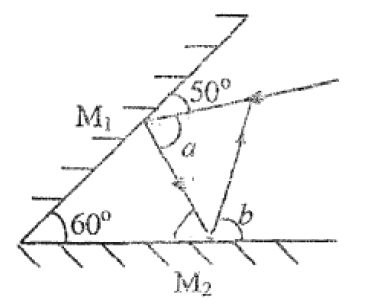
\includegraphics[width=0.4\linewidth]{assets/qdijiowqdiqwjoidjwq.png}
        
        
    \end{figure}
\end{eg}
\begin{eg}
    \begin{itemize}
        \item [sol.]
    \end{itemize}
\end{eg}

\begin{frame}{反射種類Types of reflection}
    \begin{itemize}
        \item 單向反射\\Regular reflection
        \begin{itemize}
            \item 光射向光亮的表面,例如鏡子、拋光面、平靜的水面。\\Light shines on shinny surface, such as mirror, polished surface and calm water surface.
            \item 單向反射發生時,可以看見清晰的反射影像。\\Clear image can be observed by regular reflection.
            \item 反射面的細節會較難觀察到。\\Detail of the surface is harder to observe.
        \end{itemize}
    \end{itemize}
    \begin{figure}
        \centering
        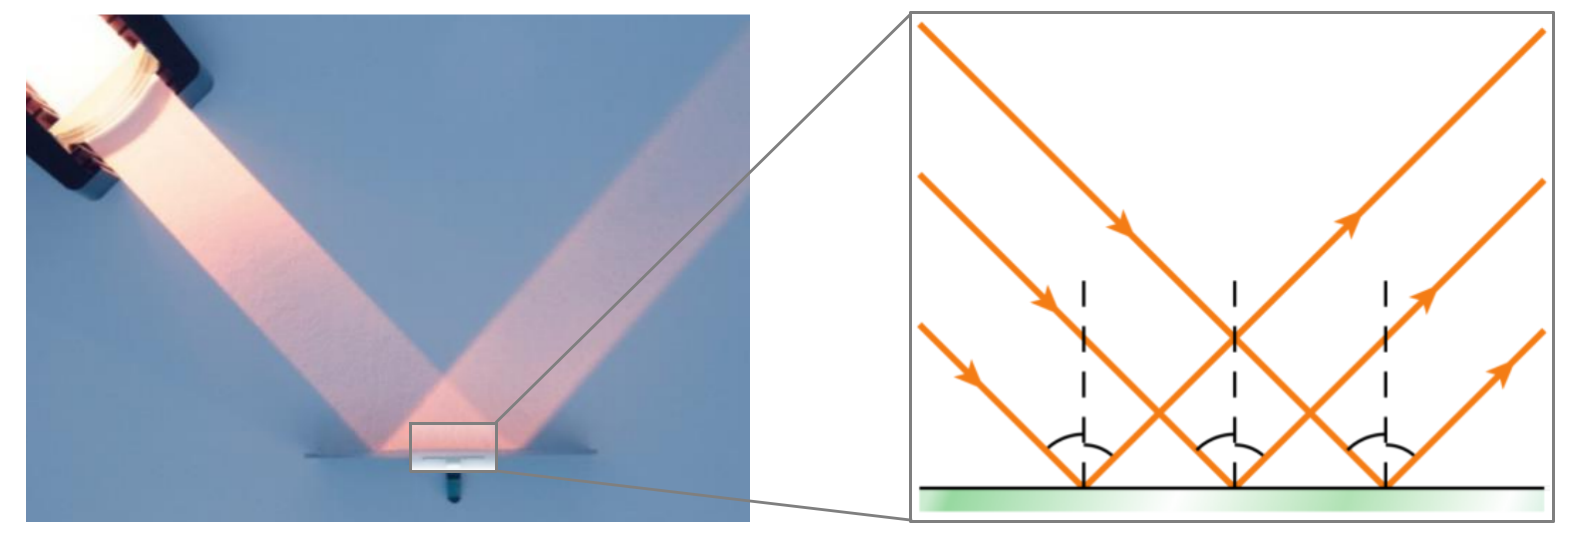
\includegraphics[width=0.75\linewidth]{assets/qdjdoiqwjoidjqwoidjqwiodjwioqjdoiqwjd.png}
    \end{figure}
\end{frame}

\begin{frame}{反射種類Types of reflection}
    \begin{itemize}
        \item 漫反射\\Diffuse reflection
        \begin{itemize}
            \item 在粗糙表面發生。例如在牆壁、黑板、白紙上。\\Occurs on rough surfaces, such as wall, blackboard and rough paper.
            \item 不能看見清晰的反射影像。\\Clear image cannot be observed by diffuse reflection.
            \item 反射面的細節會較易觀察到。\\Detail of the surface is easier to observe.
        \end{itemize}
    \end{itemize}
   \begin{figure}
       \centering
       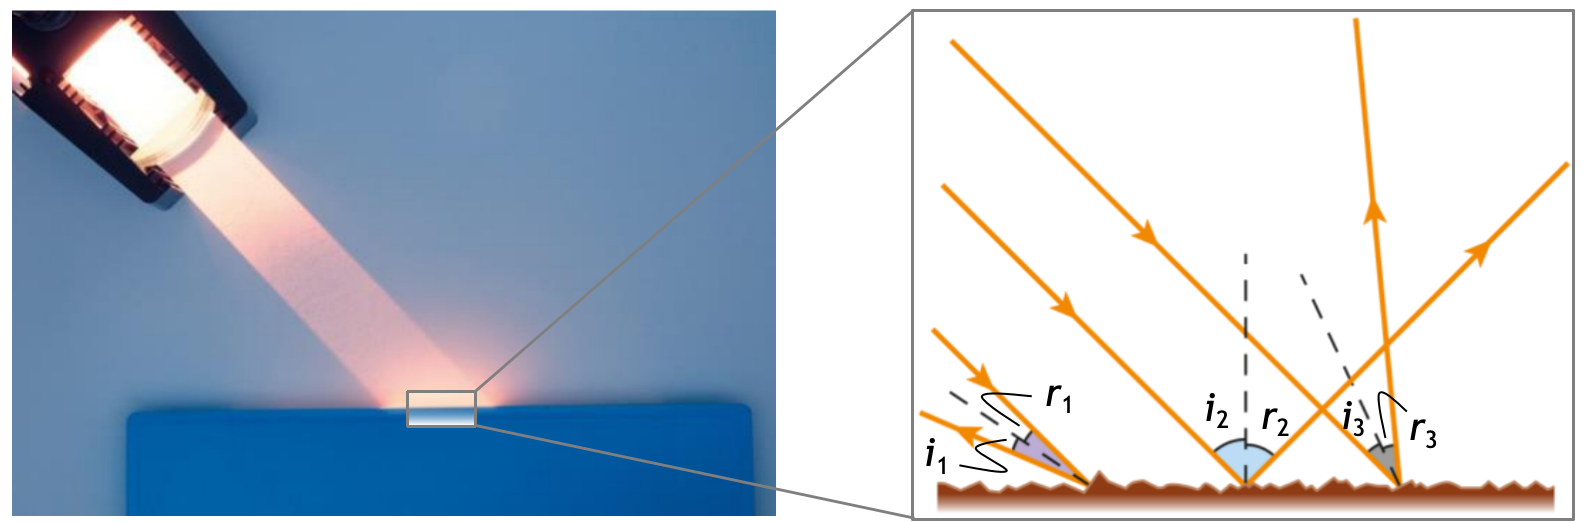
\includegraphics[width=0.75\linewidth]{assets/ddojiqwoidwqjdoijqwodjqwodjqwiodj.png}
       
       
   \end{figure}
\end{frame}

\begin{frame}{單向反射和漫反射Regular reflection and diffuse reflection}
    \begin{figure}
        \centering
        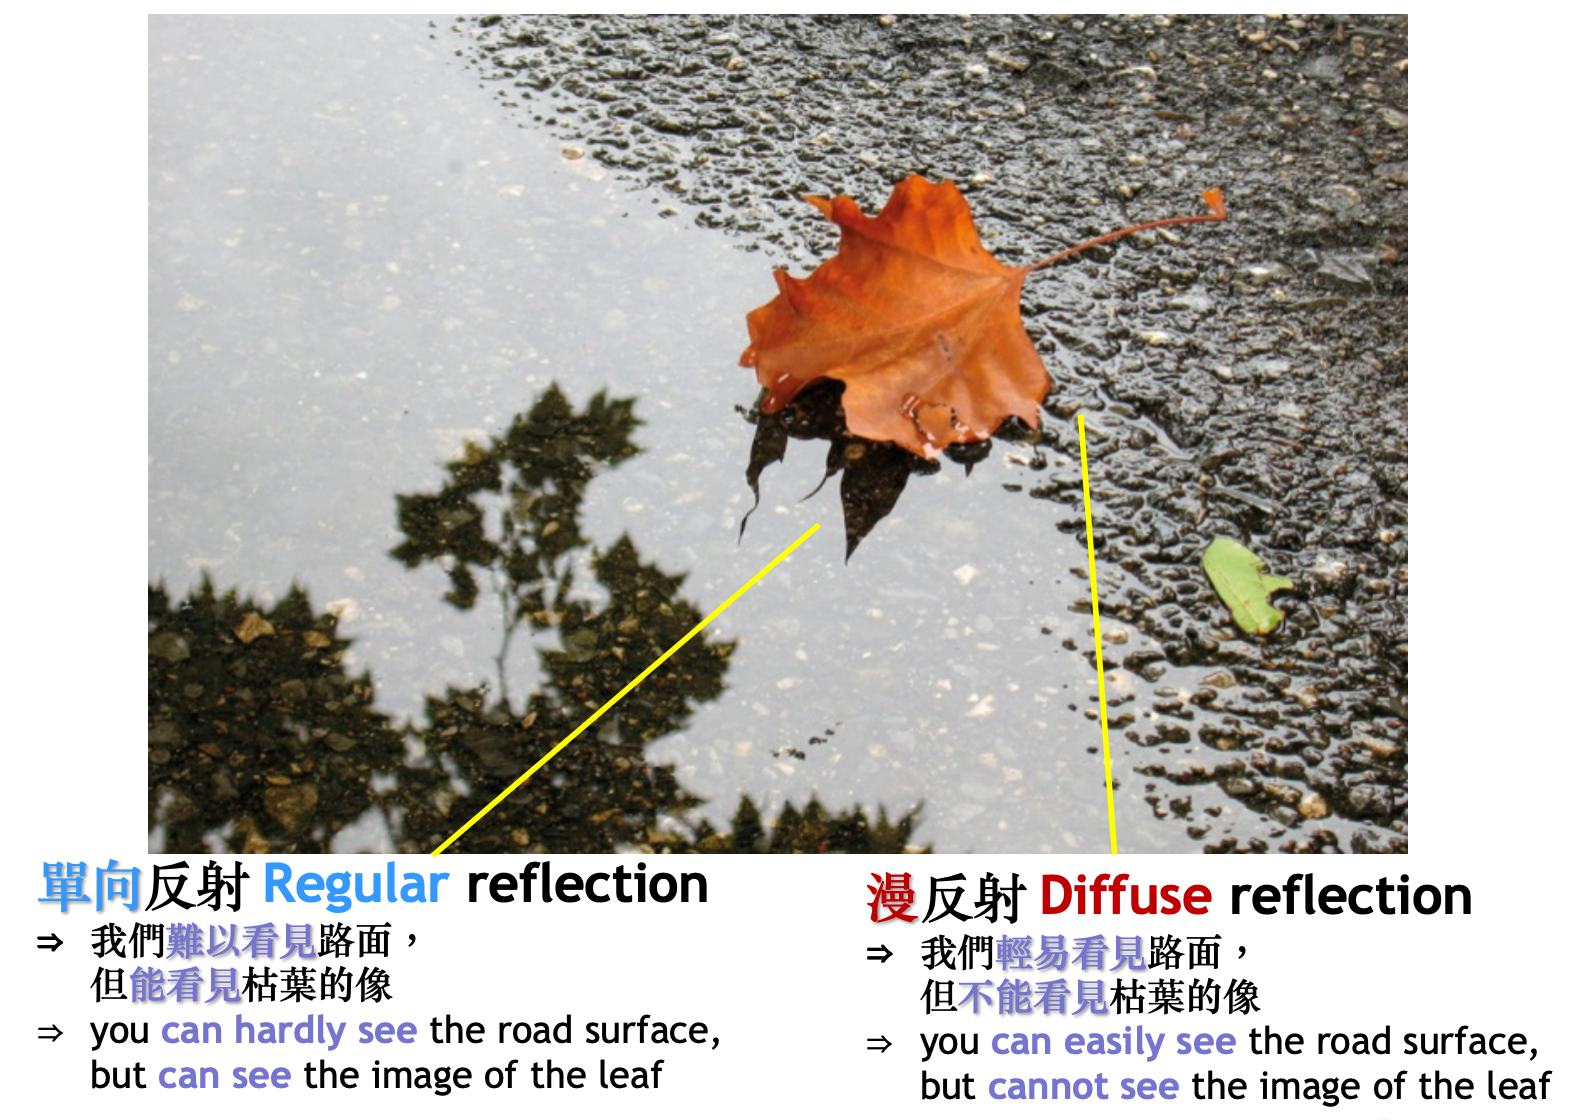
\includegraphics[width=.85\linewidth]{assets/ddjidojoidjoqiwdjqwd.png}
        
        
    \end{figure}
\end{frame}

\begin{frame}{漫反射Diffuse reflection}
    \begin{itemize}
        \item 漫反射使我們從所有方向都能看見不發光體。\\Diffuse reflection lets us see non-luminous objects from all directions.
    \end{itemize}
    \begin{figure}
        \centering
        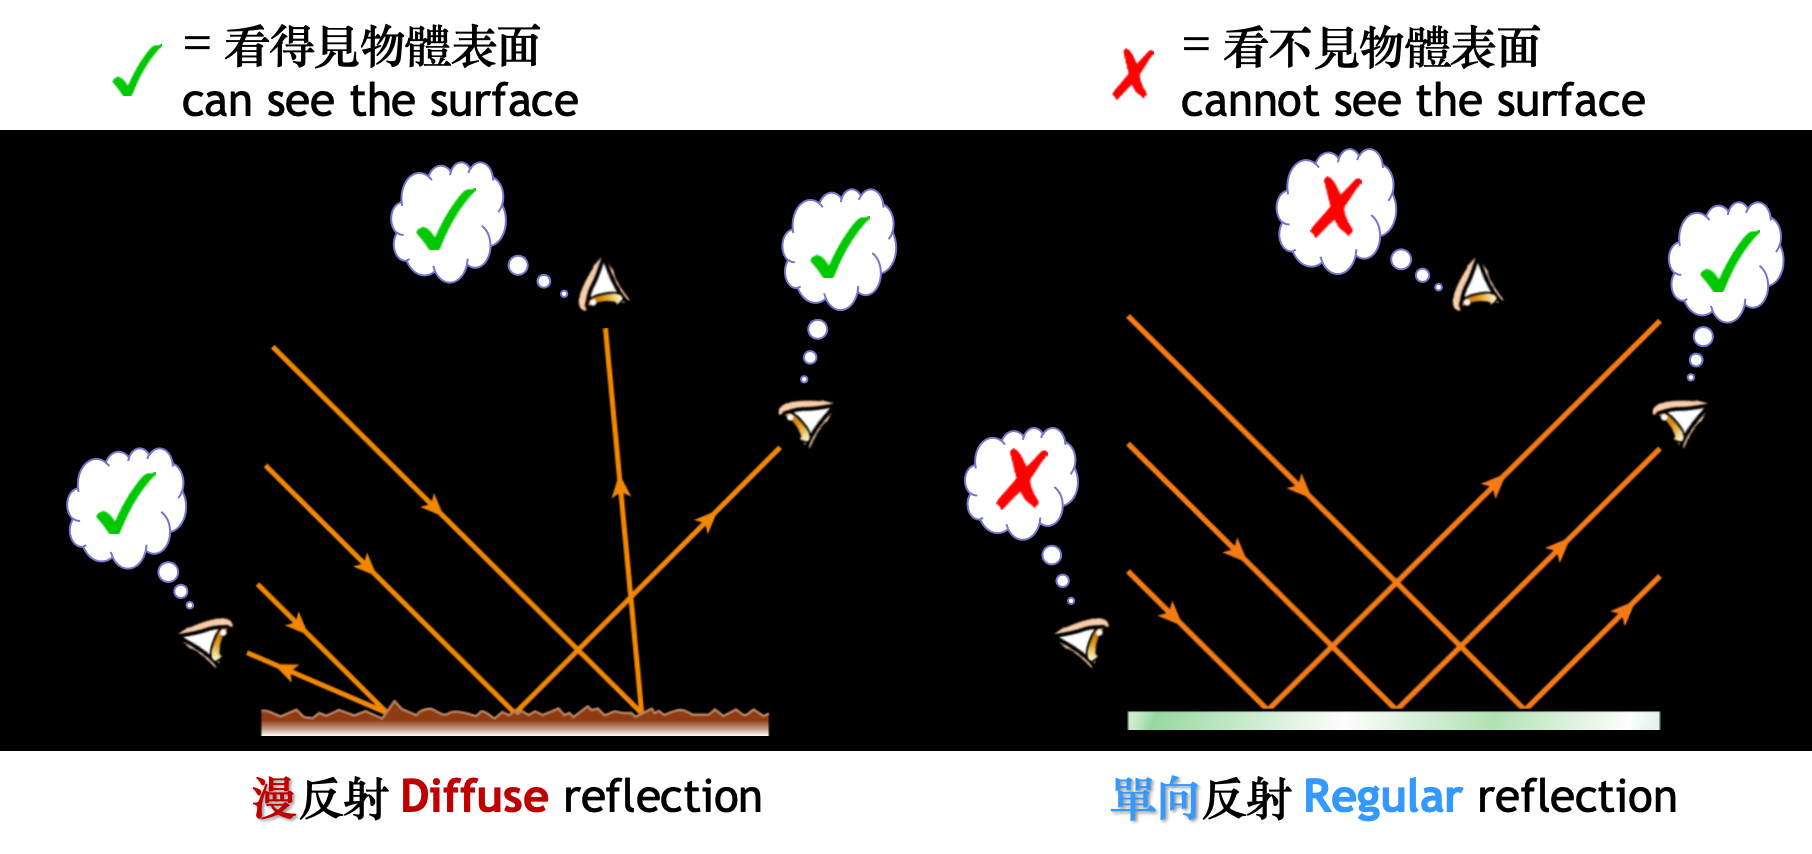
\includegraphics[width=1\linewidth]{assets/djdioqwdjqodjqwoidj.png}
        
        
    \end{figure}
\end{frame}

\begin{eg}
    在一個綿綿細雨的晚上,路面十分濕滑。約翰駕着汽車,雖然亮起了車頭燈,卻看不清前方的路面,為甚麼?\\On a rainy night, John drives his car on a wet road. He cannot see the road surface ahead clearly although the road is illuminated by the headlamps of his car. Why?
    \begin{tasks}
        \task [sol.] 從車頭燈發出的光線,在路面的積水上發生單向反射。\\
	光線並不反射回汽車的方向,約翰因而看不清路面。\par The wet road surface is smooth and flat.
	\\$\therefore$ the light from the headlamps is regularly reflected away from the car.
    \end{tasks}
\end{eg}


\begin{frame}{平面鏡Plane mirror}
    \begin{itemize}
        \item 平面鏡利用單向反射來產生清晰的、相同大小的虛像。\\A plane mirror makes use of regular reflection to give a clear image.
        \item 成像的形狀大小不受平面鏡的大小形狀影響。\\The shape and size of image are not affected by the size of mirror.
    \end{itemize}
    \begin{figure}
        \centering
        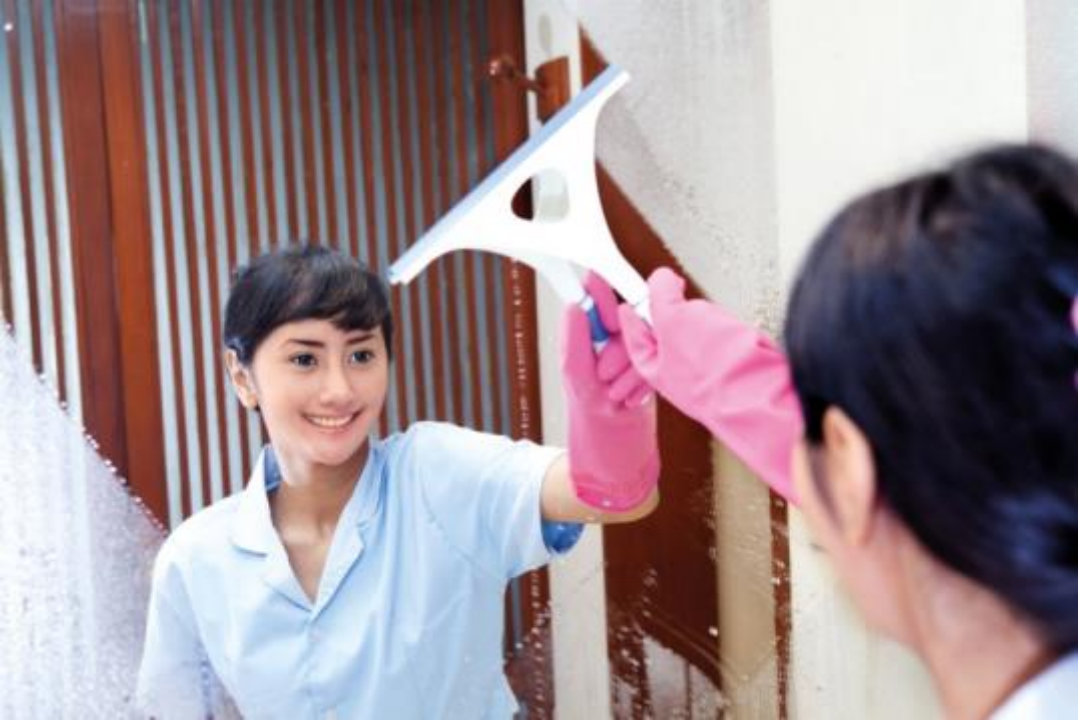
\includegraphics[width=0.5\linewidth]{assets/djwoidjwqjdioqjwodijwqoi.png}
    \end{figure}
\end{frame}



\begin{frame}{成像的特質Properties of image}
    \begin{itemize}
        \item 成像特質:\\Properties of image:
        \begin{itemize}
            \item 虛像Virtual
            \item 直立Erect/Upright
            \item 左右倒置Laterally inverted
            \item 相同大小Same size
            \item 物距$u$與像距$v$相等。\\Image distance $v$ equal to object distance $u$
        \end{itemize}
    \end{itemize}
\end{frame}

\begin{frame}{成像的一些特質Some properties of image}
    \begin{itemize}
        \item 像在鏡子後方形成。\\The image forms behind the mirror.
    \end{itemize}
\begin{figure}
    \centering
    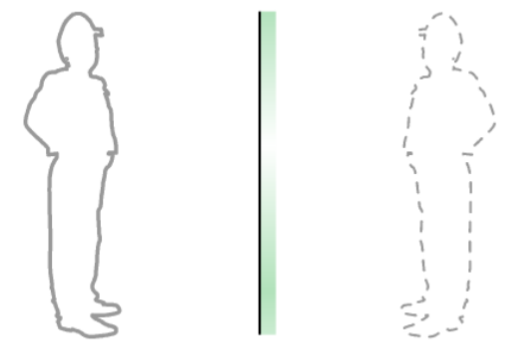
\includegraphics[width=0.5\linewidth]{assets/dqwqoi1j2w89s.png}
\end{figure}
\end{frame}

\begin{frame}{成像的一些特質Some properties of image}
\begin{itemize}
    \item 像的大小與物距無關。\\The image size is independent of the observer's location.
\end{itemize}\bigskip
    \begin{figure}
        \centering
        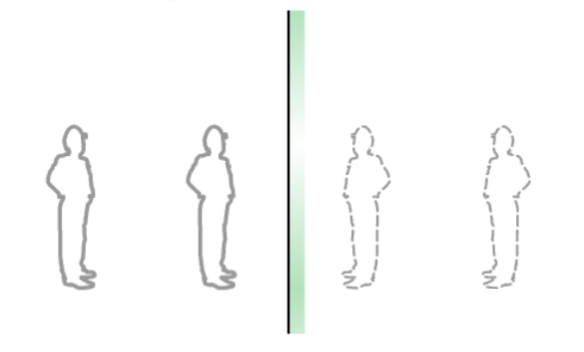
\includegraphics[width=0.6\linewidth]{assets/djoijdodoi2.png}
        
        
    \end{figure}
\end{frame}

\begin{frame}{成像的一些特質Some properties of image}
\begin{itemize}
    \item 像的大小與觀察者的位置無關。\\The image size is independent of the observer's location.
\end{itemize}
\bigskip
\begin{figure}
    \centering
    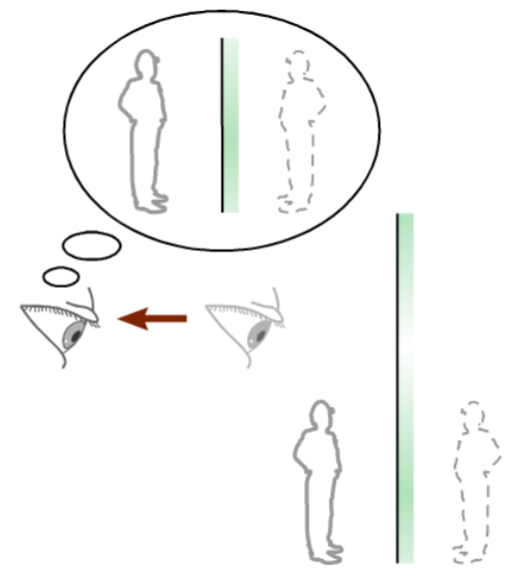
\includegraphics[width=0.35\linewidth]{assets/dqwdoji1j8n9d1u983d.png}
    
    
\end{figure}
\end{frame}



% \begin{frame}{成像的一些特質Some properties of image}

% \end{frame}

\begin{frame}{光線圖Ray diagram}
\begin{itemize}
    \item 首先,將像繪畫為與物體相同大小,並位於鏡子後方相同的距離處。\\First draw the image which is same size as the object and at the same distance behind the mirror.
    \item 所有從物體發出的光線在反射後必須看起來從影像的同一點發出。\\All the rays emitted from the object must seem to be emitted from the same point of the image after reflection.
\end{itemize}
    \begin{itemize}
        \item 實線:真實光線和實像。\\ Solid lines represent real rays and real images.
        \item 虛線:不存在的光線和虛像。\\ Dashed lines represent virtual rays and virtual images.
    \end{itemize}
    
\end{frame}


\begin{eg}
    畫出光線圖,使眼睛能看到箭咀。\\Draw a ray diagram showing how the eye can see the arrow.
    \begin{figure}
        \centering
        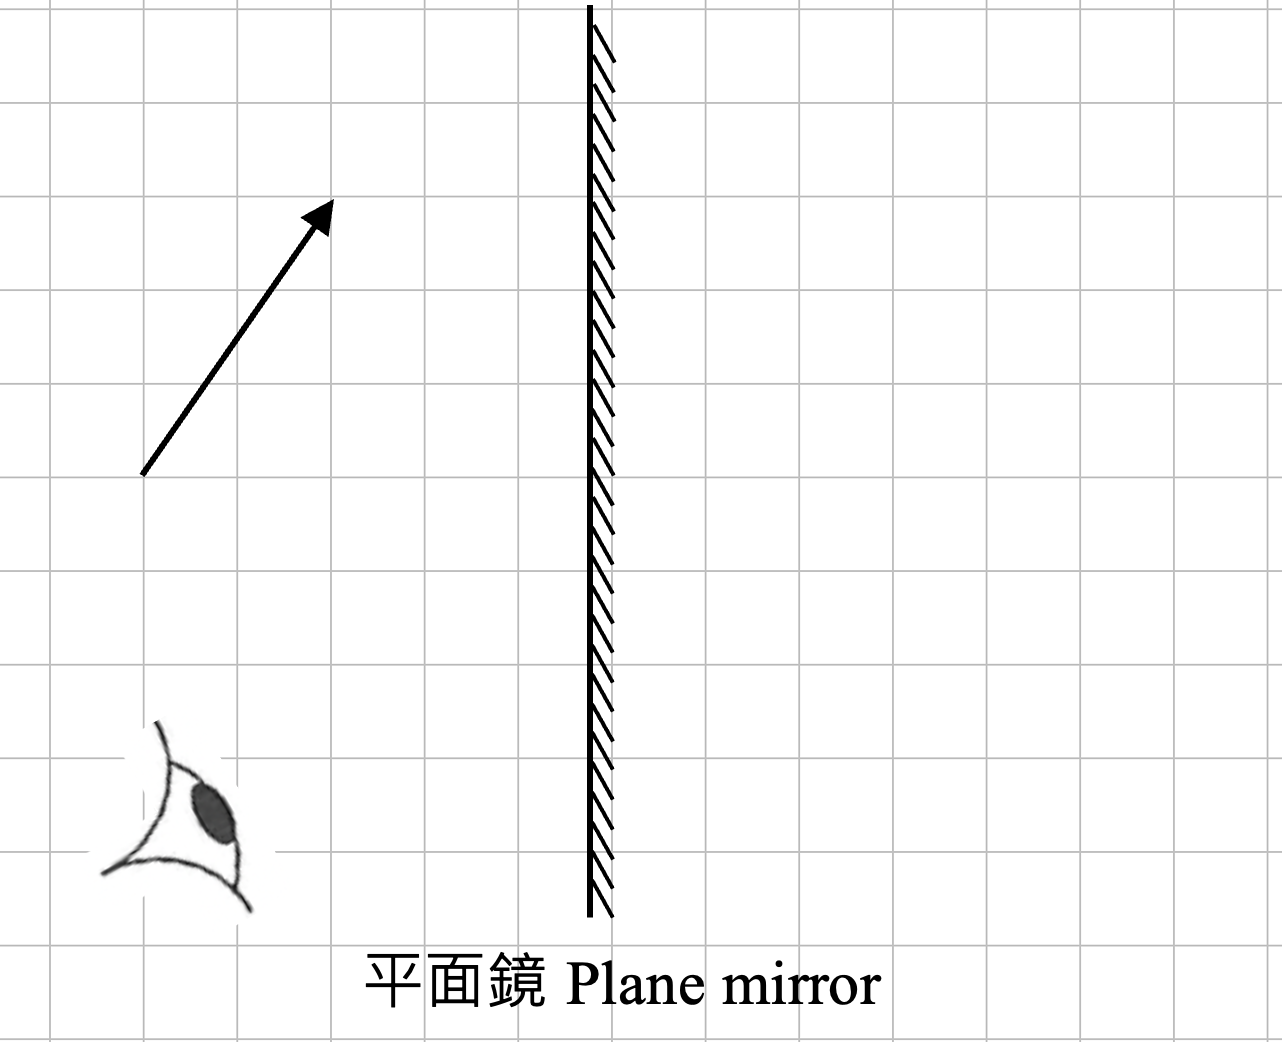
\includegraphics[width=0.75\linewidth]{assets/ddjion18uu29.png}
        
        
    \end{figure}
\end{eg}

% \begin{eg}
% 一支鉛筆放置在一個垂直的平面鏡前,如上圖所示。以下哪個選項顯示了影像的正確位置?\\A pencil is placed in front of a vertical plane mirror as shown in the figure above. Which of the following shows the correct position of the image?
%     \begin{figure}
%         \centering
%         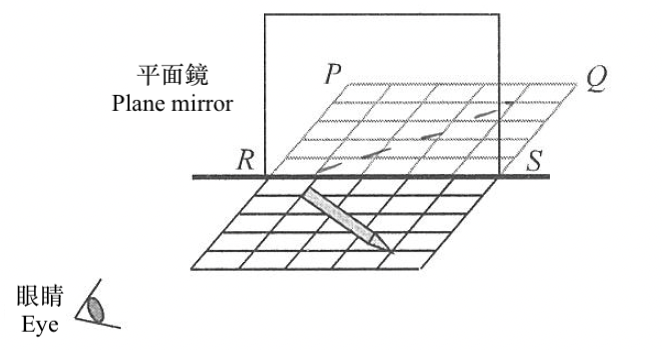
\includegraphics[width=0.5\linewidth]{assets/djiowqjdi1ge.png}
        
        
%     \end{figure}
% \end{eg}


\begin{eg}
    圖中M為一平面鏡,草繪字母F的成像。\\In the diagram, M is a plane mirror, sketch the image of F.
   \begin{figure}
       \centering
       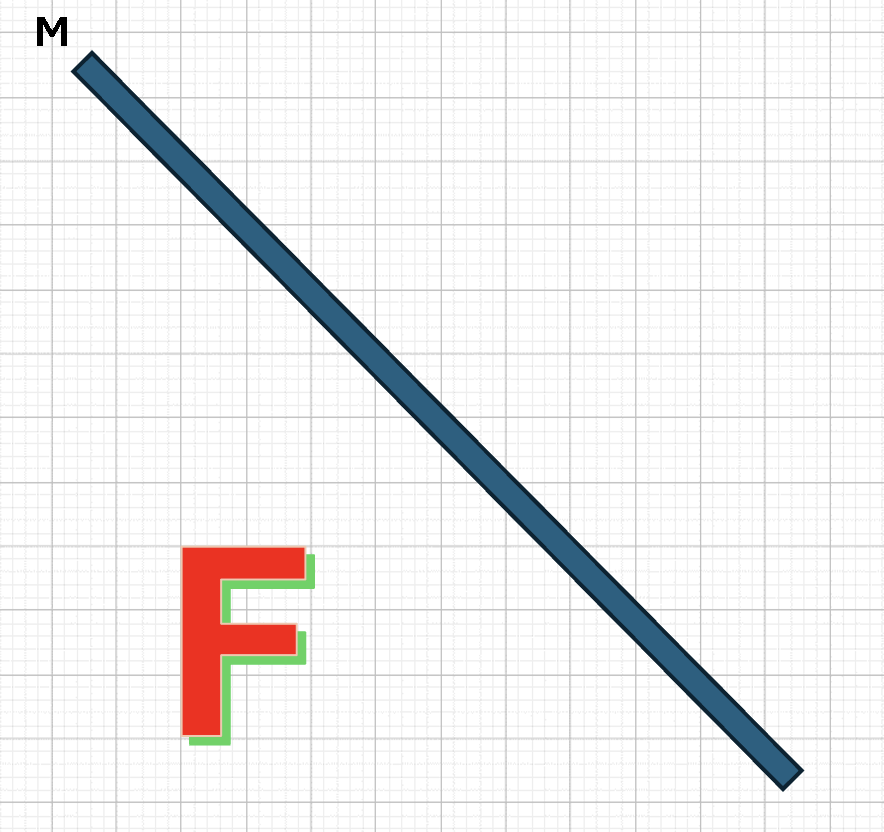
\includegraphics[width=0.5\linewidth]{assets/ddqdjioqwjdoi.png}
   \end{figure}
\end{eg}

\begin{eg}
    承上題,\\According the previous question, 
    \begin{tasks}
        \task [(a)] 若M向上移動,寫出成像的移動方向。\\Suppose M is moving upwards, write down the direction of motion of image.\vspace{1.5cm}
        \task [(b)] 若F向左移動,寫出成像的移動方向。\\Suppose is F moving left, write down the direction of motion of image.
    \end{tasks}

\end{eg}



\begin{eg}
    約瀚和瑪莉雖然素未謀面,但是他們在轉角位的鏡子中看到了對方。\\John and Mary have never met before, but at this moment they saw each other in a mirror at the street corner.\bigskip
    \begin{figure}
        \centering
        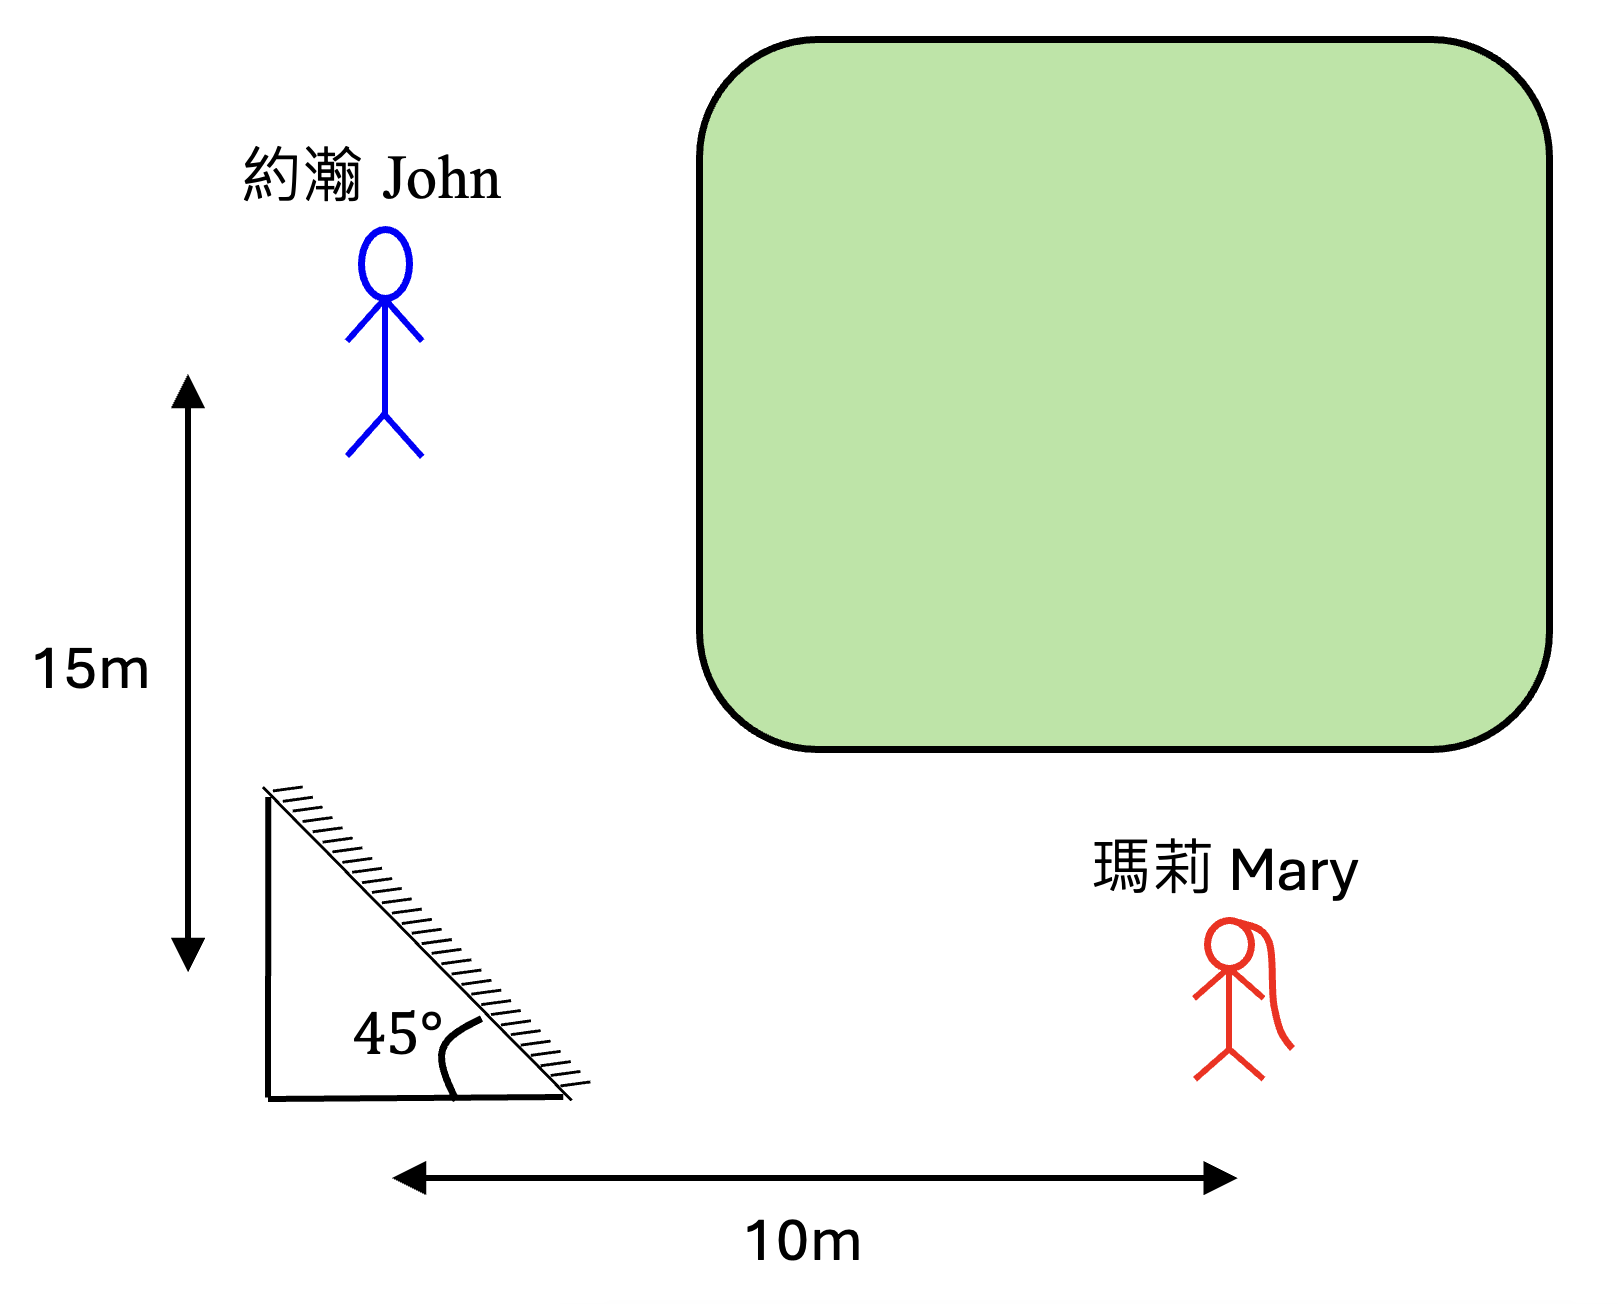
\includegraphics[width=0.55\linewidth]{assets/dwqdrcr322d.png}
        
        
    \end{figure}
    
\end{eg}
\begin{eg}
    \begin{itemize}
        \item [(a)] 從圖中畫出光線,以展示約翰如何看見瑪麗,從而繪畫出她的影像。\\Draw light rays on the figure below to show how John can see Mary and hence locate her image.
    \end{itemize}
    \begin{figure}
        \centering
        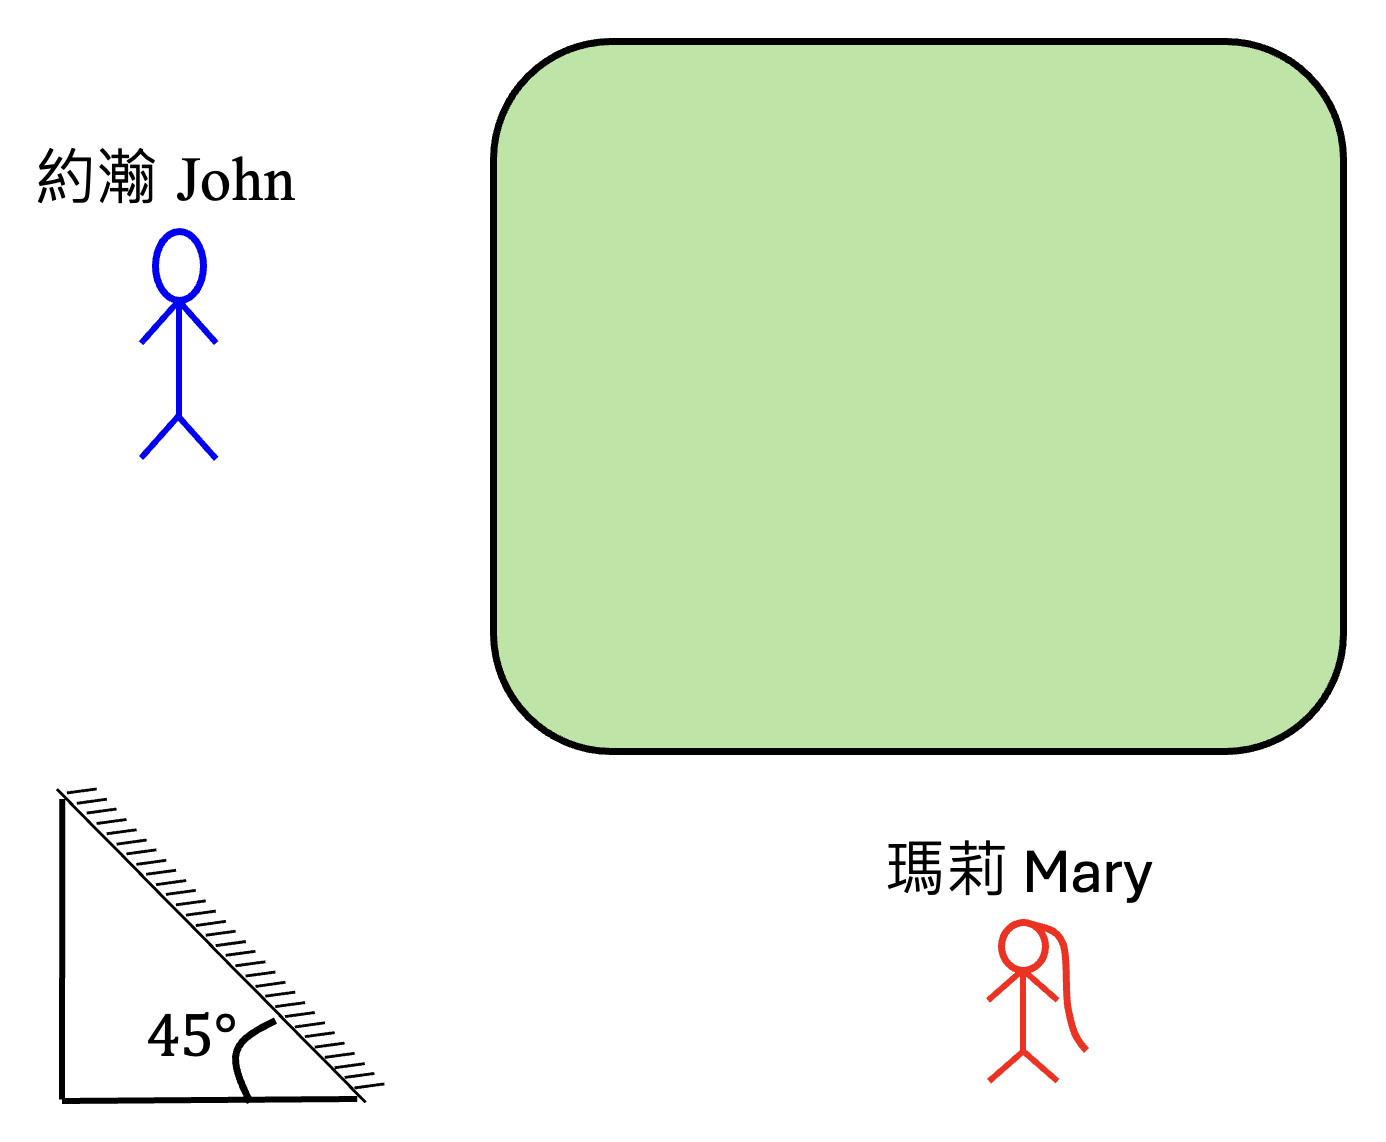
\includegraphics[width=0.4\linewidth]{assets/dewkdk21ed.png}
        
        
    \end{figure}
\end{eg}
\begin{eg}
    \begin{itemize}
        \item [(b)] 寫出約瀚和瑪莉的像之間的距離。\\Write down the distance between John and the image of Mary.\vspace{0.8cm}
        \item [(c)] 約瀚情不自禁地以\vel{5}的速率向鏡子跑去。他以多快的速率朝著瑪莉的像移動?\\John couldn't help himself and runs towards the mirror at a speed of \vel{5}. How fast does he move towards the image of Mary?\vspace{0.8cm}
        \item [(d)] 現在瑪麗也以\vel{2}的速率向鏡子移動。約翰以多快的速率朝著瑪麗的像移動?\\Now Mary is also moving towards the mirror at a speed of \vel{2}. How fast does John move towards the image of Mary?
    \end{itemize}

\end{eg}




\begin{frame}{平面鏡的最小長度Minimum length of a plane mirror}
\begin{itemize}
    \item 觀看全身像的平面鏡的最小長度,為使用者身高的一半。\\The minimum height of a full-length mirror is half the height of the user.
\end{itemize}
\begin{figure}
    \centering
    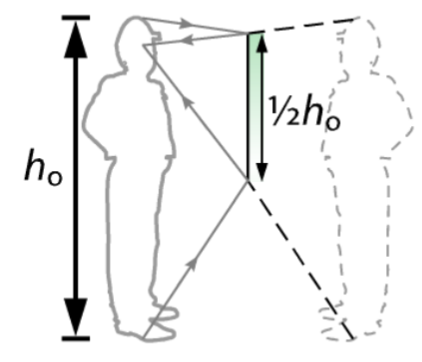
\includegraphics[width=0.4\linewidth]{assets/dq1e1.png}
\end{figure}
\end{frame}

\begin{frame}{平面鏡的最小長度Minimum length of a plane mirror}
\begin{itemize}
    \item 觀看全身像的平面鏡的最小長度與物距無關。\\The minimum height of a full-length mirror is independent of the object distance.
\end{itemize}

\begin{figure}
    \centering
    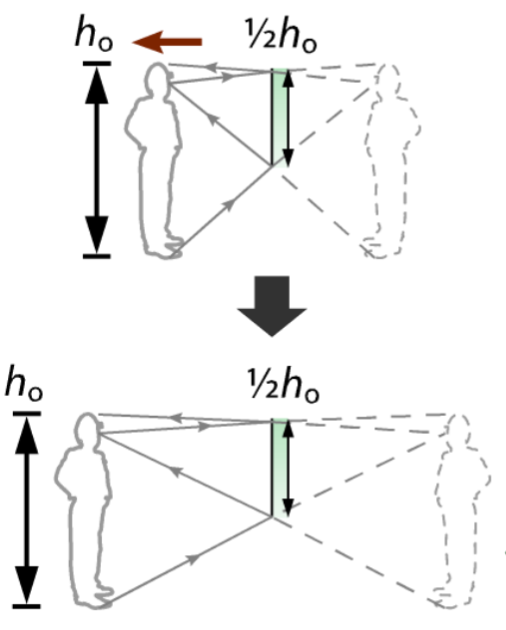
\includegraphics[width=0.4\linewidth]{assets/dwqdqop1i2m9d.png}
\end{figure}
\end{frame}

\begin{eg}
    小珍在一塊平面鏡前倒立,足尖與雙眼分別離地2.2 m 和0.6 m。 在圖中所示的一刻,她正於平面鏡前 2.0 m。\\Jane is doing handstands. Her toes and eyes are 2.2 m and 0.6 m above the floor respectively. At the instant shown, she is 2.0 m from the plane mirror.
    \begin{figure}
        \centering
        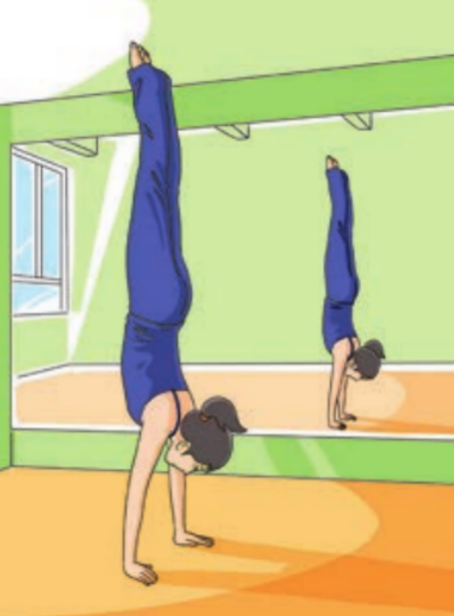
\includegraphics[width=0.25\linewidth]{assets/dwqdqwdqwd1dd3md9.png}
        
        
    \end{figure}
\end{eg}
\begin{eg}
    \begin{itemize}
        \item [(a)] 小珍與她的像相距多遠?\\How far is Jane from her image?
    \end{itemize}
\end{eg}

\begin{eg}
    \begin{itemize}
        \item [(b)] 若小珍看見自己雙手,平面鏡底邊離地的高度最大為多少?\\How far, at most, is the lower edge of the mirror from the floor so that Jane can see her hands in the mirror?
    \end{itemize}
\end{eg}

\begin{eg}
    \begin{itemize}
        \item [(c)] 若小珍看見自己的全身像,平面鏡的最小長度為多少?\\What is the minimum length of the mirror so that Jane can see her whole body in it?
    \end{itemize}

\end{eg}

\begin{eg}
    \begin{itemize}
        \item [(d)] 小珍現移至平面鏡前 0.4 m 處,(c) 部的答案會否改變?\\Jane is now 0.4 m from the mirror. Does the answer in (c) change?
    \end{itemize}
\end{eg}

\begin{eg}
在圖中,一面高度為$h$的平面鏡$MN$被安裝在垂直牆上的可調節位置。$E$是觀察者的眼睛,距離牆壁1 m,距離地面1.5 m。$PQ$是一根高3 m的垂直柱子,位於觀察者後方4 m處。觀察者透過鏡子可以看到整個柱子的影像。$h$的最小值是多少?\\In the figure, a plane mirror $MN$ of height $h$ is mounted in an adjustable vertical position on a vertical wall. $E$ is an observer's eye which is 1 m from the wall and 1.5 m above the ground. $PQ$ is a vertical post of height 3 m and is 4 m behind the observer. Looking into the mirror the observer can see the whole image of the post. What is the minimum value of $h$?
    \begin{figure}
        \centering
        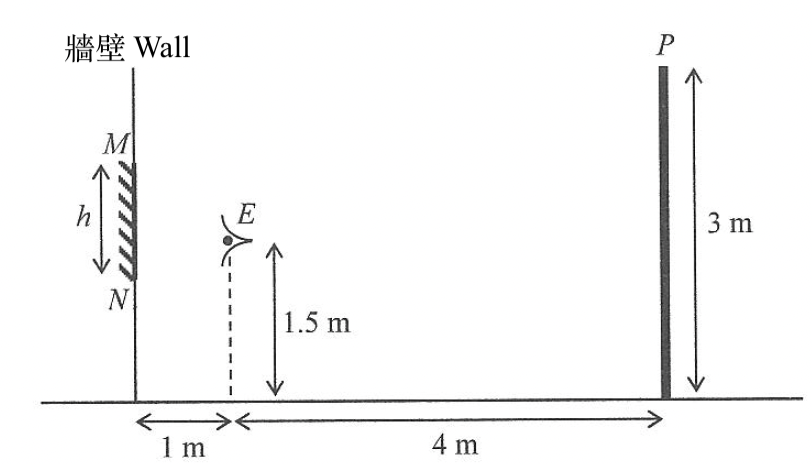
\includegraphics[width=0.4\linewidth]{assets/dwddd89u2j38d2.png}
    \end{figure}
\end{eg}

\begin{eg}
    \begin{figure}
        \centering
        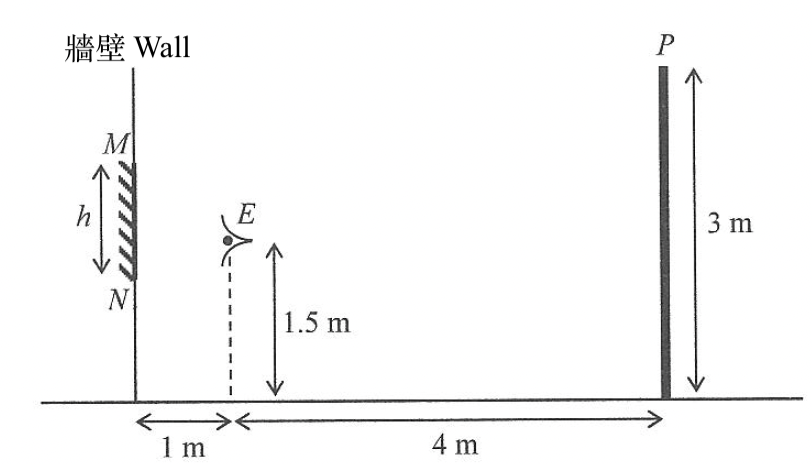
\includegraphics[width=0.5\linewidth]{assets/dwddd89u2j38d2.png}
    \end{figure}
\end{eg}

\begin{eg}
    下圖為文德的餐廳平面圖,為使店內顯得更加寬敞,他在北面的 牆壁上裝置了一塊很大的平面鏡。 當文德站於$O$點,他能從平面鏡看見南面櫥窗。櫥窗闊 5.4 m, 最接近 $O$點的一點在$O$點以東3 m。\\The figure shows the top view of Fred's restaurant. To create an illusion of space, he sets up a large mirror on the north wall. When he stands at $O$, he can see the whole south window in the mirror. The window is 5.4 m wide and 3 m from $O$ in the east direction.
    \begin{figure}
        \centering
        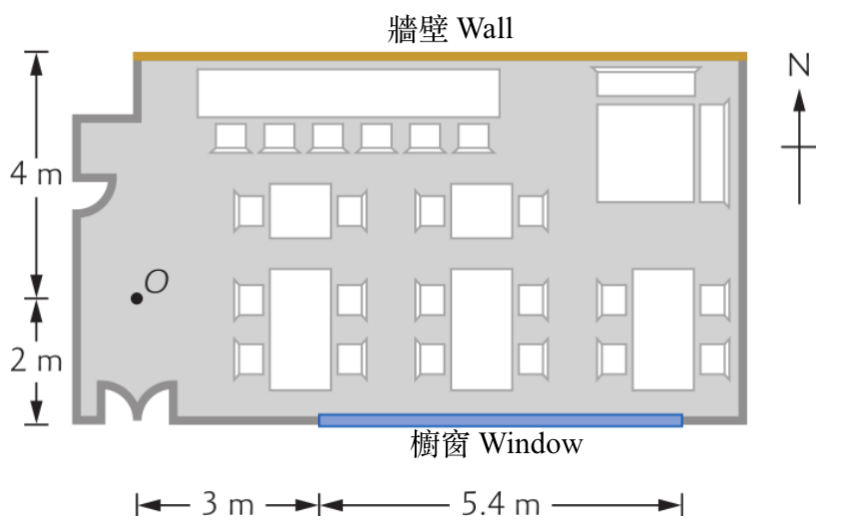
\includegraphics[width=0.5\linewidth]{assets/duq9d8qwdage.png}
    \end{figure}
\end{eg}

\begin{eg}
    \begin{itemize}
        \item [(a)] 草繪一幅光線圖,表示文德站在$O$點時,如何從平面鏡 看見整面櫥窗。把文德的眼睛視作一點。\\Sketch a ray diagram to show how Fred sees the window in the mirror when he stands at $O$. Treat his eyes as a point.
    \end{itemize}
\end{eg}

\begin{eg}
    \begin{itemize}
        \item [(b)] 北面的平面鏡最小闊度 w 應為多少?\\What is the minimum width w of the north mirror?
    \end{itemize}
\end{eg}

\begin{eg}
    \begin{itemize}
        \item [(c)] 若文德向北移數步,(b) 部的答案(即 w)會如何改變?\\How does the answer in (b) change (i.e. w) if Fred moves a few steps due north?
    \end{itemize}

\end{eg}

\begin{eg}
    \begin{itemize}
        \item [(d)] 若文德向東移數步,(b) 部的答案(即 w) 會如何改變?\\How does the answer in (b) change (i.e. w) if Fred moves a few steps due east?
    \end{itemize}

\end{eg}

\begin{frame}{平面鏡的缺點Disadvantages of plane mirror}
    \begin{itemize}
        \item 平面鏡會產生多重反射,造成複像。\\Plane mirror has multiple reflections to give multiple images.
        \begin{itemize}
            \item 觀察到的成像會較不清晰。\\The image observed would then become less clear.
        \end{itemize}
    \end{itemize}\bigskip
    
    \begin{figure}
        \centering
        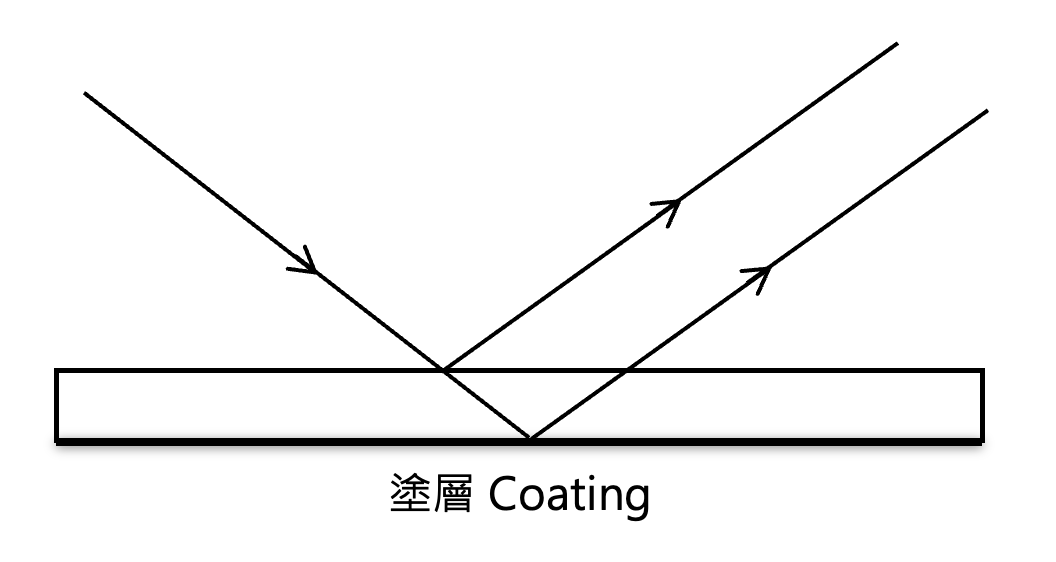
\includegraphics[width=0.5\linewidth]{assets/idjnqjdiqjndqdo189d9nn18u982.png}
    \end{figure}
    
\end{frame}



\begin{frame}{潛望鏡Periscope}
    \begin{itemize}
        \item 用來觀察不同高度的物件。\\To view objects at different levels.
    \end{itemize}\bigskip
    \begin{figure}
        \centering
        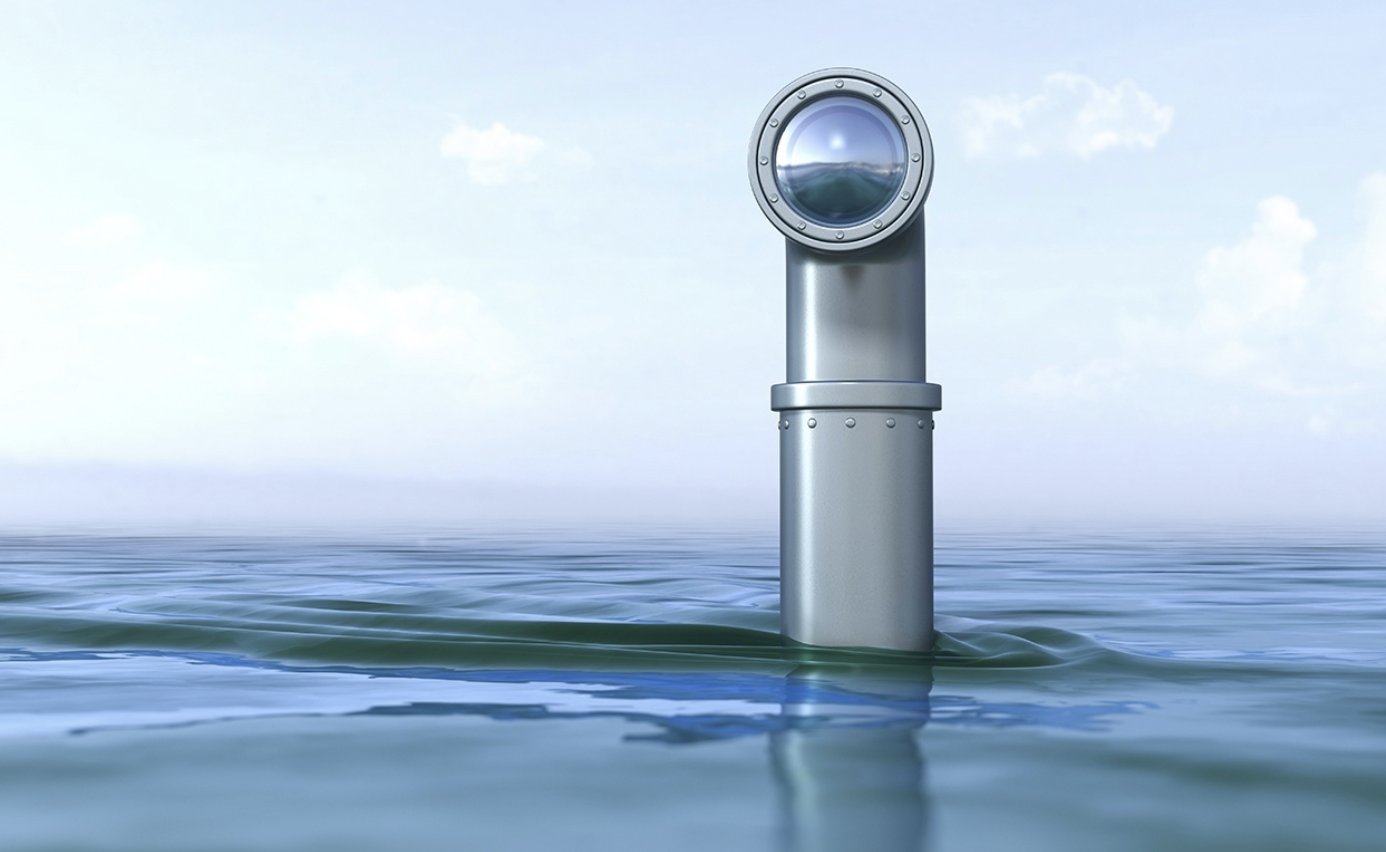
\includegraphics[width=0.5\linewidth]{assets/dqdjiwmage.png}
    \end{figure}
\end{frame}





\begin{frame}{潛望鏡Periscope}
    \begin{itemize}
        \item 左邊潛望鏡生成的虛像是直立,沒有左右倒置。\\Virtual image formed by left periscope is erect and not laterally inverted.
        \item 右邊潛望鏡生成的虛像是上下倒置,沒有左右倒置。\\Virtual image formed by right periscope is upside down and not laterally inverted.
    \end{itemize}
    \begin{figure}
        \centering
        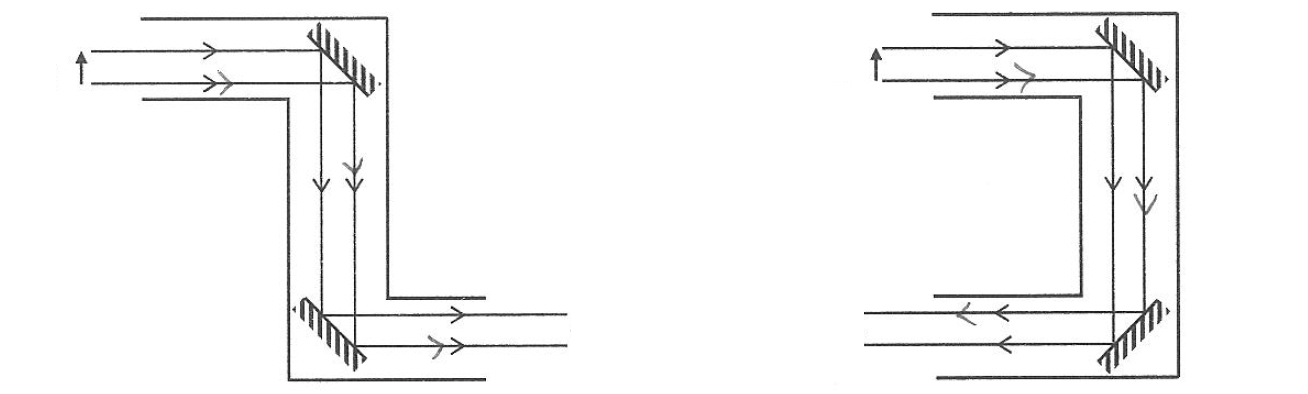
\includegraphics[width=1\linewidth]{assets/dw109id099m0e.png}

    \end{figure}
\end{frame}

% \begin{eg}
%     圖示一學生所設計的潛望鏡,並用以觀察一物體。試草繪學生所看到的像。\\The figure shows a periscope designed by a student for observing an object. Sketch the image that the student would see.
%     \medskip
%         {\par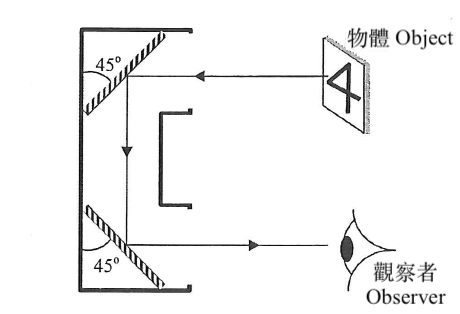
\includegraphics[width=0.6\linewidth]{assets/hduhewdewid1213123141.png}\par}
% \end{eg}

\begin{eg}
    % 這位學生修改了他的設計,如圖所示,這位學生能看到怎樣的像?\\This student modifies his setup as shown, what would be the image that the student can see?
    圖示一學生所設計的潛望鏡,並用以觀察一物體。試草繪學生所看到的像。\\The figure shows a periscope designed by a student for observing an object. Sketch the image that the student would see.
    \medskip
        {\par
    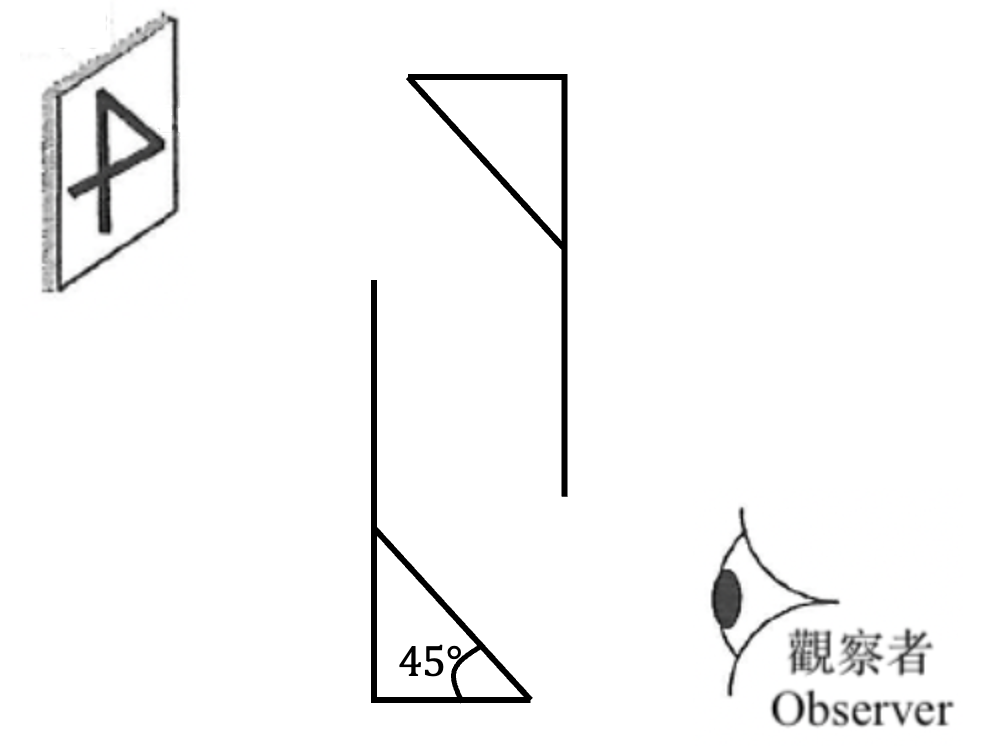
\includegraphics[width=0.6\linewidth]{assets/ddqwdoqk.png}
  \par}
\end{eg}

\begin{eg}
    文浩透過一個潛望鏡觀察一個玩具士兵$O$。潛望鏡中的兩塊平面 鏡相距 20 cm,文浩的眼睛 $E$ 在頂部的平面鏡 $M_2$前10 cm,而玩 具士兵則位於底部的一塊平面鏡$M_1$前15 cm。求文浩的眼睛與平 面鏡$M_2$中的玩具士兵成像的距離。\\Michael is viewing a toy soldier $O$ through a periscope whose two plane mirrors are 20 cm apart. His eye $E$ is 10 cm in front of the upper mirror $M_2$, While the toy soldier is 15 cm in front of the lower mirror $M_1$. How far is the image of the toy soldier produced by $M_2$ from Michael's eye?
    \begin{figure}
        \centering
        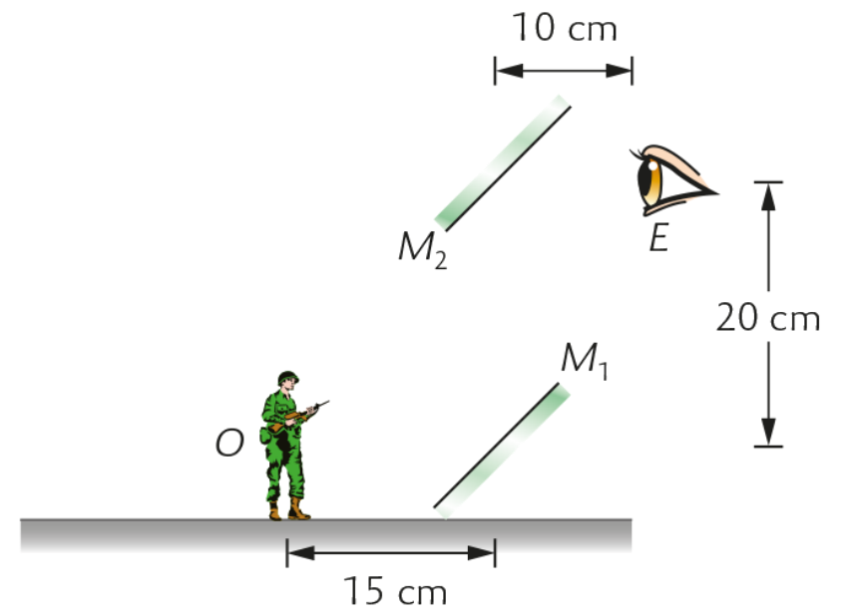
\includegraphics[width=0.4\linewidth]{assets/dwdwe1age.png}
    \end{figure}
\end{eg}

\begin{eg}
    \begin{figure}
        \centering
        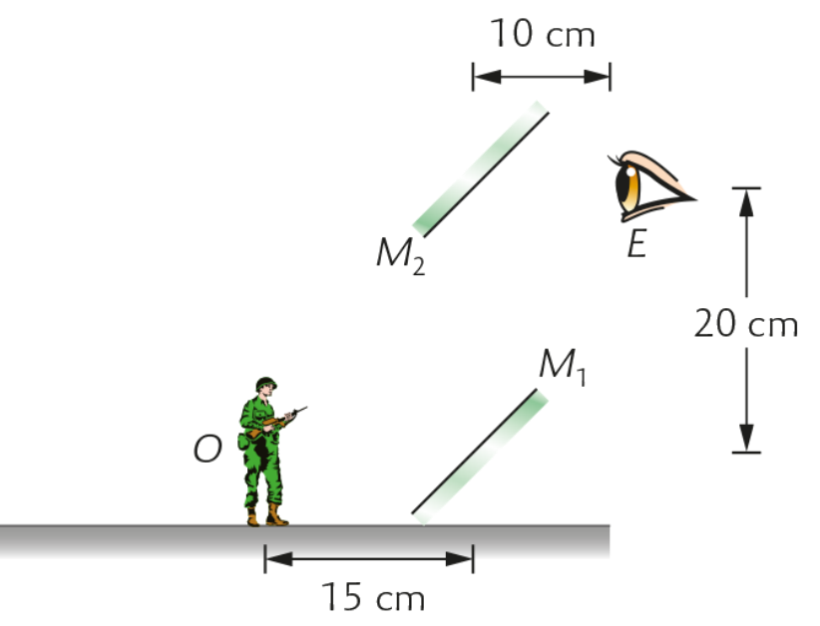
\includegraphics[width=0.5\linewidth]{assets/dq1asd.png}
    \end{figure}
\end{eg}



\begin{frame}{後視鏡Rear-view mirror}
    \begin{itemize}
        \item 令司機能看見背後的乘客或交通情況。\\Allow drivers to see the passengers or traffic conditions behind.
    \end{itemize}\bigskip
    \begin{figure}
        \centering
        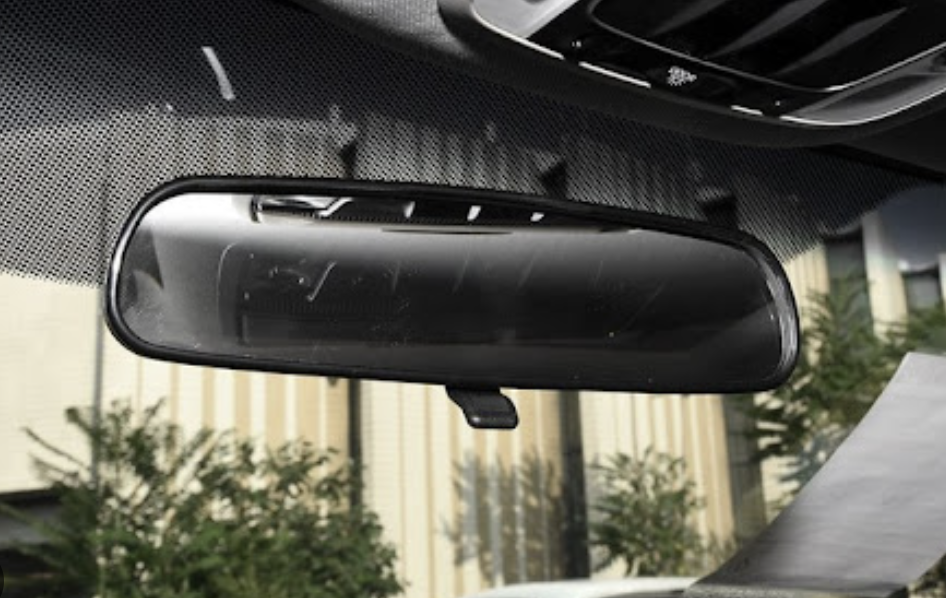
\includegraphics[width=0.5\linewidth]{assets/idjioq8jd9d.png}
        
        
    \end{figure}
\end{frame}

\begin{frame}{後視鏡Rear-view mirror}
    \begin{figure}
        \centering
        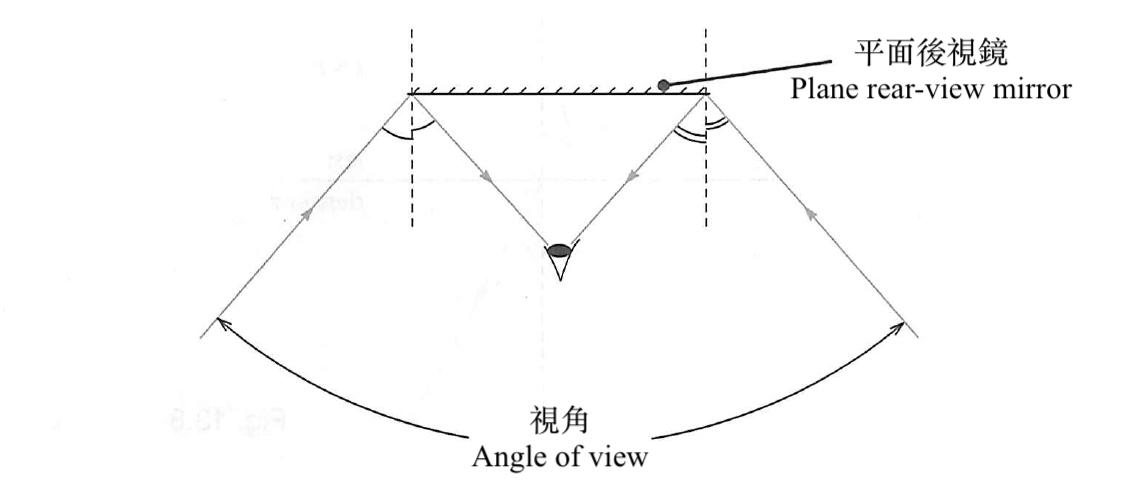
\includegraphics[width=\linewidth]{assets/dqjioj98dun89n9821.png}
        
        
    \end{figure}
\end{frame}

\begin{frame}{多重影像Multiple images}
    \begin{figure}
        \centering
        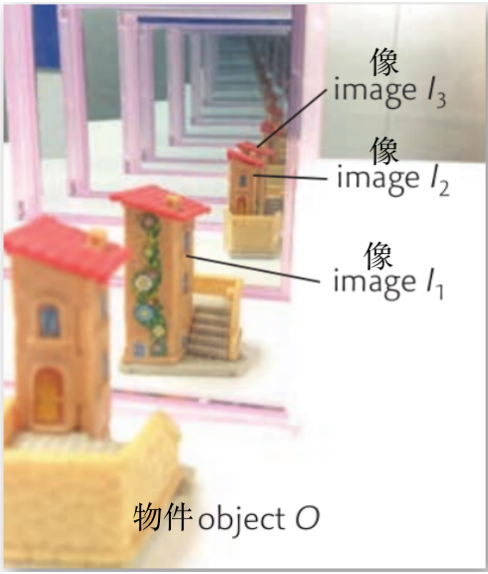
\includegraphics[width=0.5\linewidth]{assets/ddkopdk.png}
    \end{figure}
\end{frame}

\begin{frame}{多重影像Multiple images}
    \begin{itemize}
        \item 其中一方鏡子的像在另一方的鏡子形成像,因此會生成很多的像。\\The image from one side of mirror forms an image on the other side, and so on, therefore plenty of images can be seen.
        \item 越遠的像不是越緊靠在一起。兩個相鄰的單數(或雙數)像總是有固定的距離。\\The distance between two successive odd (or even) images is always the same.
    \end{itemize}
    
    \begin{figure}
        \centering
        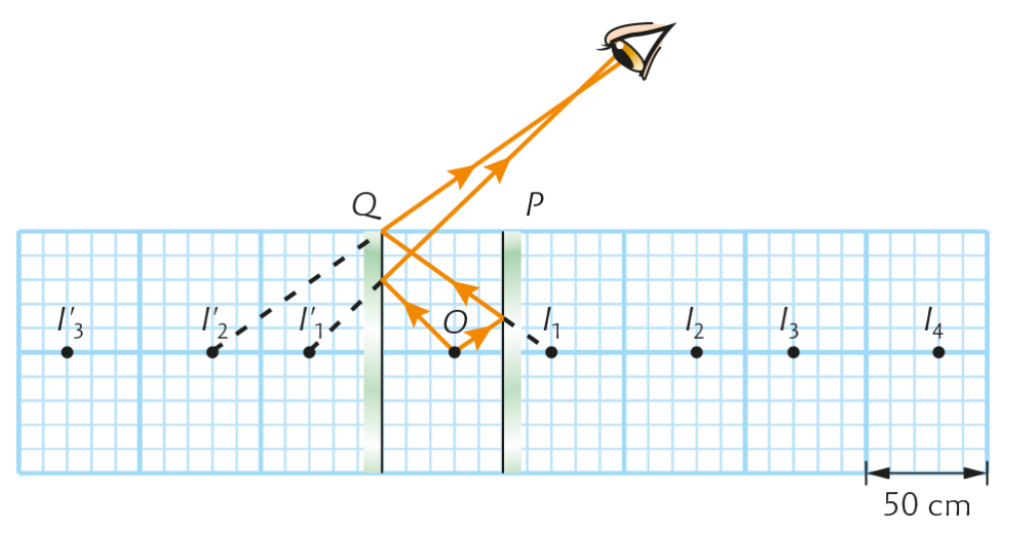
\includegraphics[width=0.66\linewidth]{assets/ddqjoij12.png}
        
        
    \end{figure}
\end{frame}

\begin{eg}
    兩塊平面鏡$P$和$Q$ 相對而立,兩者相距 50 cm,一件細小的玩具$O$放在平面鏡 $P$ 前 20 cm。把玩具視作一點。\\Two parallel plane mirrors $P$ and $Q$ are separated by 50 cm. An object $O$ is placed 20 cm in front of $P$. Treat the object as a point.
    \begin{figure}
        \centering
        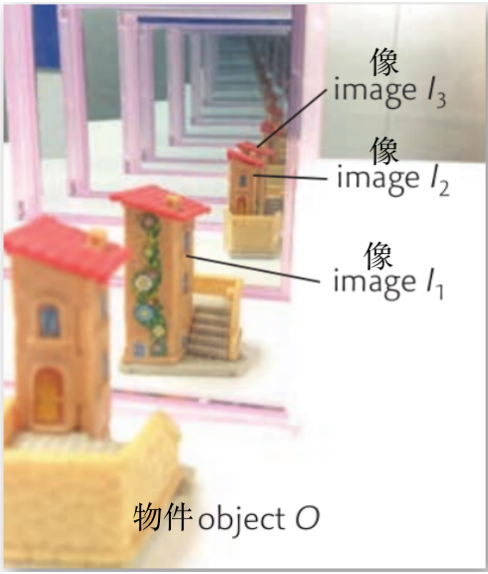
\includegraphics[width=0.3\linewidth]{assets/ddkopdk.png}
    \end{figure}
\end{eg}

\begin{eg}
    \begin{itemize}
        \item [] 像 $I_4$ 和玩具相距多遠?\\How far is image $I_4$ from the object?
    \end{itemize}\bigskip
\begin{figure}
        \centering
        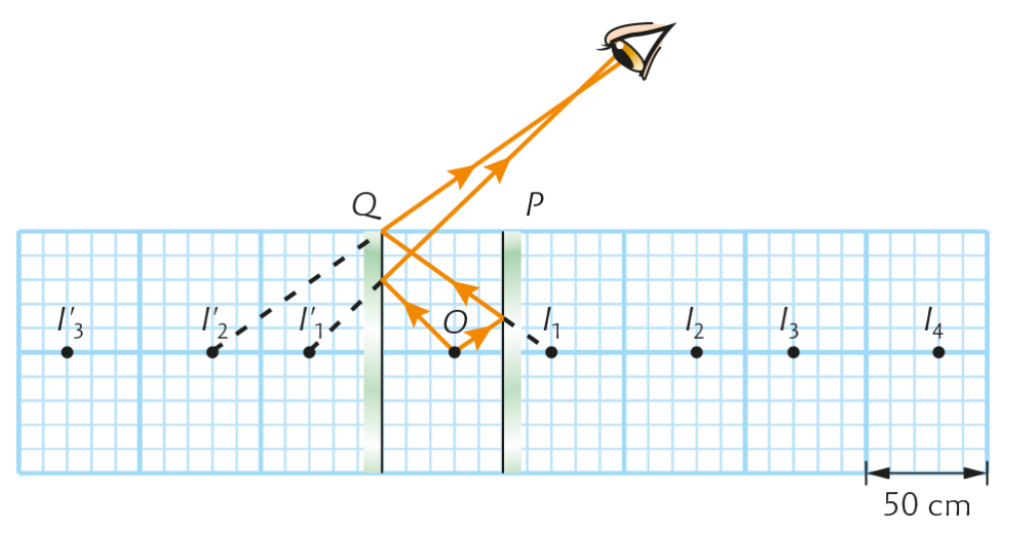
\includegraphics[width=0.75\linewidth]{assets/ddqjoij12.png}
        
        
    \end{figure}
\end{eg}

\begin{frame}{FYI}
    \begin{figure}
        \centering
        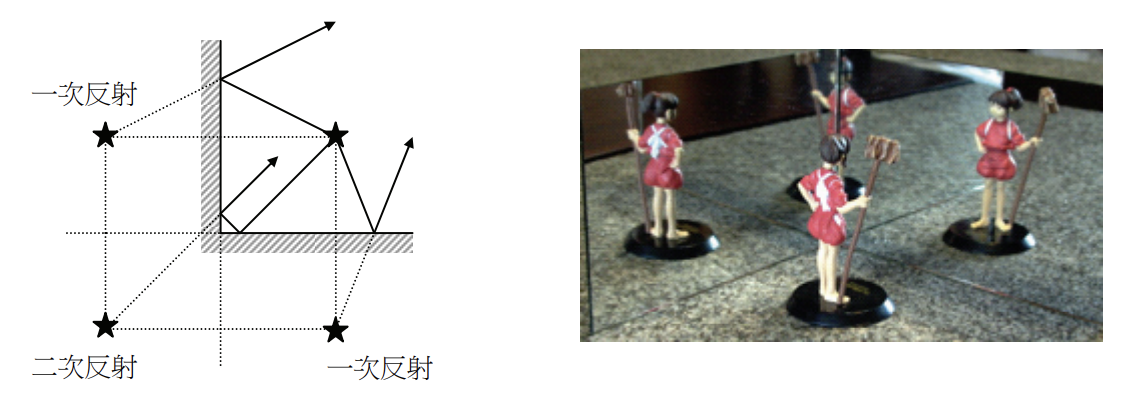
\includegraphics[width=\linewidth]{assets/dj98qwu.png}
        
        
    \end{figure}
\end{frame}












































































































\end{document}